%% \documentclass[compress,12pt]{beamer}

%% \usepackage{mathrsfs}
%% \usepackage{stmaryrd} % \llbracket

%% \newcommand{\bv}[1]{{\boldsymbol{#1}}}

%% % This puts serifs on equations, which is not standard in Beamer talks.
%% % \usefonttheme[onlymath]{serif}

%% \usetheme{Darmstadt} % Berlin with no bottom nav and rounded blocks, pretty nice, a bit too much at top though
%% \usecolortheme{sidebartab}

%% \usepackage{times}
%% \usepackage{units}

%% \setbeamercovered{invisible}
%% \logo{
\includegraphics[width=.5in]{figures/word3}}

%% \title{Using LibMesh for Scientific Computations}
%% \subtitle{\url{https://github.com/libMesh/libmesh}}
%% \author{Roy Stogner \and John Peterson}
%% \date{November 3, 2005}
%% \institute{EM 397.4 -- Grid Generation \& Adaptive Grids}

%% \begin{document}

%% \begin{frame}
%%   \titlepage
%% \end{frame}



%% %%%%%%%%%%%%%%%%%%%%%%%%%%%%%%%%%%%%%%%%%%%%%%%%%%%%%%%%%%%%%%%%%%%%%%%%%%%%%%%
%% \begin{frame}{Outline}
%%   \begin{itemize}
%%     \item A Model Problem
%%     \item Galerkin FE Method
%%     \item Penalty Boundary Conditions
%%     \item Adaptivity
%%     \item Error Indicators
%%     \item 1D Example
%%   \end{itemize}
%% \end{frame}

\frame
{
  \Large
  \begin{block}{}
    \center{\bf Adaptive Mesh Refinement}
  \end{block}
}



%%%%%%%%%%%%%%%%%%%%%%%%%%%%%%%%%%%%%%%%%%%%%%%%%%%%%%%%%%%%%%%%%%%%%%%%%%%%%%%
\section{Adaptive Mesh Refinement}
\begin{frame}{Model Problem}
\begin{itemize}
  \item Consider the 1D model ODE
    \begin{equation}
      \left\{
	\begin{array}{ccc}
	  -u'' + bu' +cu &=& f \hspace{.25in} \in \hspace{.1in} \Omega = (0,L) \\
	  u(0) =  u_0   && \\
	  u(L) =  u_L	&&
	\end{array}
	\right.
    \end{equation}

  \item with weak form
    \begin{equation}
      \int_{\Omega} \left( u' v' + b u' v + cuv \right) \; dx = \int_{\Omega} fv \; dx
    \end{equation}

    for every $v \in H^1_0 (\Omega)$.
\end{itemize}
\end{frame}


%%%%%%%%%%%%%%%%%%%%%%%%%%%%%%%%%%%%%%%%%%%%%%%%%%%%%%%%%%%%%%%%%%%%%%%%%%%%%%%
\begin{frame}{Model Problem (cont.)}
\begin{itemize}
\item The analogous $d$-dimensional problem with $\Omega \subset \mathbb{R}^d$
  and boundary $\partial \Omega$ is
    \begin{equation}
      \left\{
	\begin{array}{ccl}
	  -\Delta u + \bv{b} \cdot \nabla u + cu &=& f
	  \hspace{.25in} \in \hspace{.1in} \Omega  \\
	  \phantom{-\Delta u + \bv{b} \cdot \nabla u + c}u & = & g
	  \hspace{.25in} \in \hspace{.1in} \partial \Omega
	\end{array}
	\right.
    \end{equation}

  \item with weak form
    \begin{equation}
      \int_{\Omega} \left( \nabla u \cdot \nabla v + (\bv{b} \cdot \nabla u) v + cuv \right) \; dx = \int_{\Omega} fv \; dx
    \end{equation}

\end{itemize}

\end{frame}


%%%%%%%%%%%%%%%%%%%%%%%%%%%%%%%%%%%%%%%%%%%%%%%%%%%%%%%%%%%%%%%%%%%%%%%%%%%%%%%
\begin{frame}{Model Problem (cont.)}
\begin{itemize}
\item The finite element method works with the weak form, replacing the trial and
  test functions $u,v$ with their approximations $u^h, v^h$, and summing the
  contributions of the element integrals
  \gdef\eqneltint{      \sum_{e=1}^{N_e} \int_{\Omega_e}
      \left( \nabla u^h \cdot \nabla v^h + (\bv{b} \cdot \nabla u^h) v^h + cu^h v^h
      -fv^h \right)\;  dx=0}
    \begin{equation}\label{eqn:element_integrals}
      \eqneltint
    \end{equation}

  \item Remark: We considered here a standard piecewise continuous finite element basis.
    In general, $\nabla u^h$ will have a jump discontinuity across element boundaries.
\end{itemize}
\end{frame}



%%%%%%%%%%%%%%%%%%%%%%%%%%%%%%%%%%%%%%%%%%%%%%%%%%%%%%%%%%%%%%%%%%%%%%%%%%%%%%%
\begin{frame}{Galerkin FE Method}
\begin{itemize}
  \item Expressing $u^h$ and $v^h$ in our chosen piecewise continuous polynomial
    basis
    \begin{equation}
      u^h = \sum_{j=1}^{N} u_j \varphi_j \hspace{1in} v^h = \sum_{i=1}^{N} c_i \varphi_i
    \end{equation}
    we obtain on each element $\Omega_e$
    \begin{equation}
      \small
      \sum_{j=1}^{N} u_j \left[ \int_{\Omega_e} \left( \nabla \varphi_j \cdot \nabla \varphi_i +
      (\bv{b} \cdot \nabla \varphi_j) \varphi_i + c \varphi_j \varphi_i \right) dx \right] =
      \int_{\Omega_e} f \varphi_i \; dx
    \end{equation}
    for $i=1 \ldots N$.

  \item In the standard element-stiffness matrix form,
    \begin{equation}
      \bv{K_e}\bv{U} = \bv{F_e}
    \end{equation}

\end{itemize}
\end{frame}


%%%%%%%%%%%%%%%%%%%%%%%%%%%%%%%%%%%%%%%%%%%%%%%%%%%%%%%%%%%%%%%%%%%%%%%%%%%%%%%
\begin{frame}{LibMesh Representation}
\begin{itemize}
  \item To code the model problem in \texttt{LibMesh}, the user must provide the
    routine which computes $\bv{K_e}$ and $\bv{F_e}$ for each element.

  \item The integrals are computed over the reference element using an appropriate
    numerical quadrature rule with weights $w_q$ and points $\bv{\xi}_{q}$,  $q=1 \ldots N_{q}$.
    \begin{equation}
      \int_{\Omega_e} f \varphi_i \; dx =
      \int_{\hat{\Omega}_e} f \varphi_i \; |J| d\xi \approx
      \sum_{q=1}^{N_q} w_q |J(\bv{\xi}_q)| f(\bv{\xi}_q) \varphi_i(\bv{\xi}_q)
      \end{equation}
\end{itemize}
\end{frame}


\begin{frame}{LibMesh Representation (cont.)}
\begin{itemize}
  \item \texttt{LibMesh} provides the following variables for constructing
    $\bv{K_e}$ and $\bv{F_e}$ at quadrature point \texttt{q}:
    \begin{itemize}
      \item \texttt{JxW[q]} = the scalar value of the element Jacobian map times the
	quadrature rule weight
      \item \texttt{phi[i][q]}  = $\varphi_i(\bv{\xi}_{q})$
      \item \texttt{dphi[i][q]} = $(J^{-1} \cdot \nabla_{\bv{\xi}} \varphi_i) (\bv{\xi}_{q})$
	(e.g. in 1D, this is $\frac{\partial \phi_i}{\partial \xi}\frac{\partial \xi}{\partial x}(\xi_q)$)
    \end{itemize}
\end{itemize}
\end{frame}



%%%%%%%%%%%%%%%%%%%%%%%%%%%%%%%%%%%%%%%%%%%%%%%%%%%%%%%%%%%%%%%%%%%%%%%%%%%%%%%
\begin{frame}[fragile]{LibMesh Representation (cont.)}
\small
\begin{semiverbatim}
  for (q=0; q<Nq; ++q) \{
    // Compute b, c, f at this quadrature point
    // ...

    for (i=0; i<N; ++i) \{
      Fe(i)   += JxW[q]*f*phi[i][q];

      for (j=0; j<N; ++j)
        Ke(i,j) += JxW[q]*(
          (dphi[i][q]*dphi[j][q])  +
          (b*dphi[j][q])*phi[i][q] +
           c*phi[j][q]*phi[i][q]
                          );
    \}
  \}
\end{semiverbatim}

\end{frame}


%%%%%%%%%%%%%%%%%%%%%%%%%%%%%%%%%%%%%%%%%%%%%%%%%%%%%%%%%%%%%%%%%%%%%%%%%%%%%%%
\begin{frame}{Boundary Conditions}
  \begin{itemize}
  \item Dirichlet boundary conditions are typically enforced after
    the global stiffness matrix $\bf{K}$ has been assembled
    %from the element connectivity and the
    %element stiffness matrices $\bf{K_e}$
  \item This usually involves
    \begin{enumerate}
    \item placing a ``1'' on the main diagonal of the
      global stiffness matrix
    \item zeroing out the row entries
    \item placing the Dirichlet
      value in the rhs vector
    \item subtracting off the column entries from the rhs
    \end{enumerate}
  \end{itemize}
  \begin{equation}
    \nonumber
      \begin{bmatrix}
	k_{11} & k_{12} & k_{13} & .  \\
	k_{21} & k_{22} & k_{23} & .  \\
	k_{31} & k_{32} & k_{33} & .  \\
	  .    &   .    &    .   & .
      \end{bmatrix},
      \begin{bmatrix}
	f_{1}  \\
	f_{2}  \\
	f_{3}  \\
	  .
      \end{bmatrix} \rightarrow
      \begin{bmatrix}
	1      & 0      & 0      & 0  \\
	0      & k_{22} & k_{23} & .  \\
	0      & k_{32} & k_{33} & .  \\
	  0    &   .    &    .   & .
      \end{bmatrix},
      \begin{bmatrix}
	g_{1}  \\
	f_{2} - k_{21}g_1  \\
	f_{3} - k_{31}g_1  \\
	  .
      \end{bmatrix}
  \end{equation}
\end{frame}


%%%%%%%%%%%%%%%%%%%%%%%%%%%%%%%%%%%%%%%%%%%%%%%%%%%%%%%%%%%%%%%%%%%%%%%%%%%%%%%
\begin{frame}{Boundary Conditions (cont.)}
  \begin{itemize}
    \item This approach works for an interpolary finite element basis
      but not in the general case.

    \item For large problems with parallel sparse matrices, it
      is inefficient to change individual entries once the global matrix is assembled.

    \item What is required is a way to enforce boundary conditions for
      a generic finite element basis \emph{at the element stiffness matrix level}.

    \item A Solution: ``Penalty'' Boundary Conditions
      \begin{itemize}
      \item \emph{For many years, penalty boundary conditions were the preferred approach in \libMesh{}, so you may encounter them.}
      \end{itemize}
  \end{itemize}
\end{frame}


%%%%%%%%%%%%%%%%%%%%%%%%%%%%%%%%%%%%%%%%%%%%%%%%%%%%%%%%%%%%%%%%%%%%%%%%%%%%%%%
\begin{frame}{Penalty Boundary Conditions}
  \begin{itemize}
  \item An additional ``penalty'' term is added to the standard weak form
    \begin{equation}
      \nonumber
      \scriptsize
      \int_{\Omega} \left( \nabla u \cdot \nabla v + (\bv{b} \cdot \nabla u) v + cuv \right) dx
      + \underbrace{\frac{1}{\epsilon} \int_{\partial \Omega} (u-g)v \; dx}_{\text{penalty term}} =
      \int_{\Omega} fv \; dx
    \end{equation}

  \item Here $\epsilon \ll 1$ is chosen so that, in floating point arithmetic,
    $\frac{1}{\epsilon} + 1 = \frac{1}{\epsilon}$.

  \item This weakly enforces $u=g$ on the boundary at the element level, and works for
    general finite element bases.  This approach only impacts elements who have a face 
    on the boundary of the domain.
  \end{itemize}
\end{frame}





%%%%%%%%%%%%%%%%%%%%%%%%%%%%%%%%%%%%%%%%%%%%%%%%%%%%%%%%%%%%%%%%%%%%%%%%%%%%%%%
\begin{frame}[fragile]{LibMesh Representation}

\texttt{LibMesh} provides:
\begin{itemize}
  \item A quadrature rule with \texttt{Nqf} points and \texttt{JxW\_f[]}
  \item A finite element coincident with the boundary face that has \texttt{Nf}
    shape function values \texttt{phi\_f[][]}
  %\item \texttt{penalty} = $\frac{1}{\epsilon}$
\end{itemize}
\scriptsize
\begin{semiverbatim}
for (qf=0; qf<Nqf; ++qf) \{
  // Compute g at this face quadrature point

  for (i=0; i<Nf; i++) \{
    Fe(i) += JxW_f[qf]*penalty*g*phi_face[i][qf];

    for (j=0; j<Nf; j++)
      Ke(i,j) += JxW_f[qf]*penalty*phi_f[i][qf]*phi_f[j][qf];
  \}
\}
\end{semiverbatim}

\end{frame}




%%%%%%%%%%%%%%%%%%%%%%%%%%%%%%%%%%%%%%%%%%%%%%%%%%%%%%%%%%%%%%%%%%%%%%%%%%%%%%%
\begin{frame}{Adaptivity And Error Indicators}
  \begin{itemize}

  \item A major goal of the \texttt{LibMesh} library is to provide:
    \begin{itemize}
    \item Adaptive mesh refinement support for standard geometric elements
    \item Generic, physics-independent error indicators
  \end{itemize}

  \item In this context, we'll discuss
    \begin{itemize}
    \item ``Natural'' refinement patterns
    \item A flux-jump error indicator
  \end{itemize}


  \end{itemize}
\end{frame}




%%%%%%%%%%%%%%%%%%%%%%%%%%%%%%%%%%%%%%%%%%%%%%%%%%%%%%%%%%%%%%%%%%%%%%%%%%%%%%%
\begin{frame}{Natural Refinement Patterns}
  \begin{tabular}{ccc}\\
    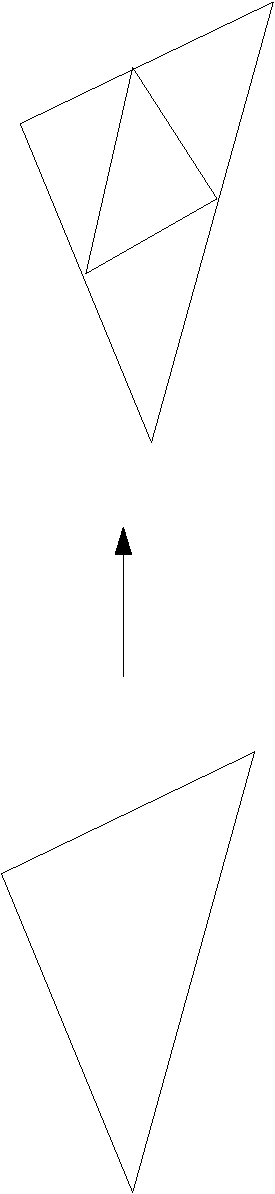
\includegraphics[angle=-90, width=.45\textwidth]{amr/triangle_refinement} &&
    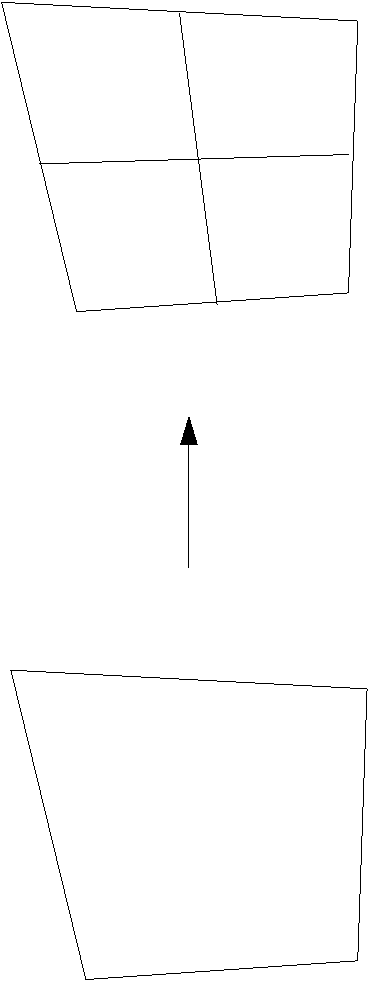
\includegraphics[angle=-90, width=.45\textwidth]{amr/quad_refinement} \\
    Triangle && Quadrilateral \\
    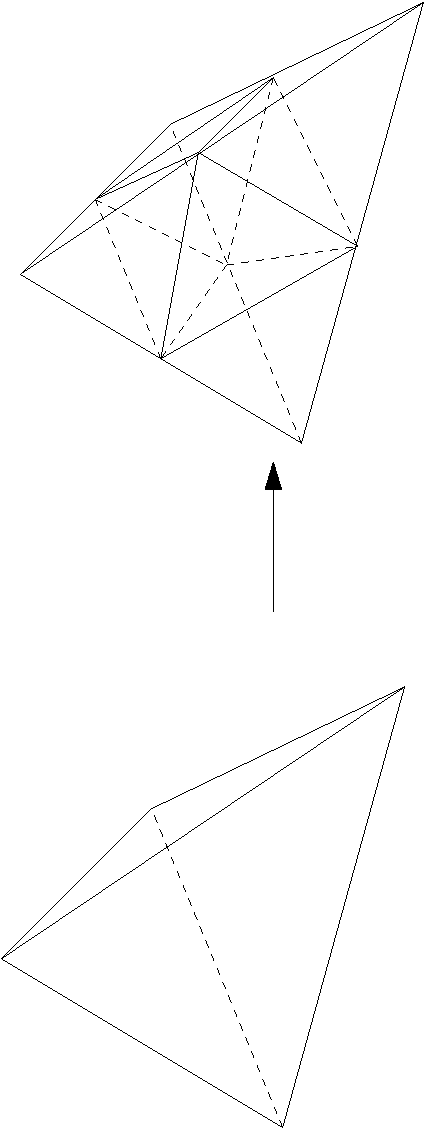
\includegraphics[angle=-90, width=.45\textwidth]{amr/tet_refinement} &&
    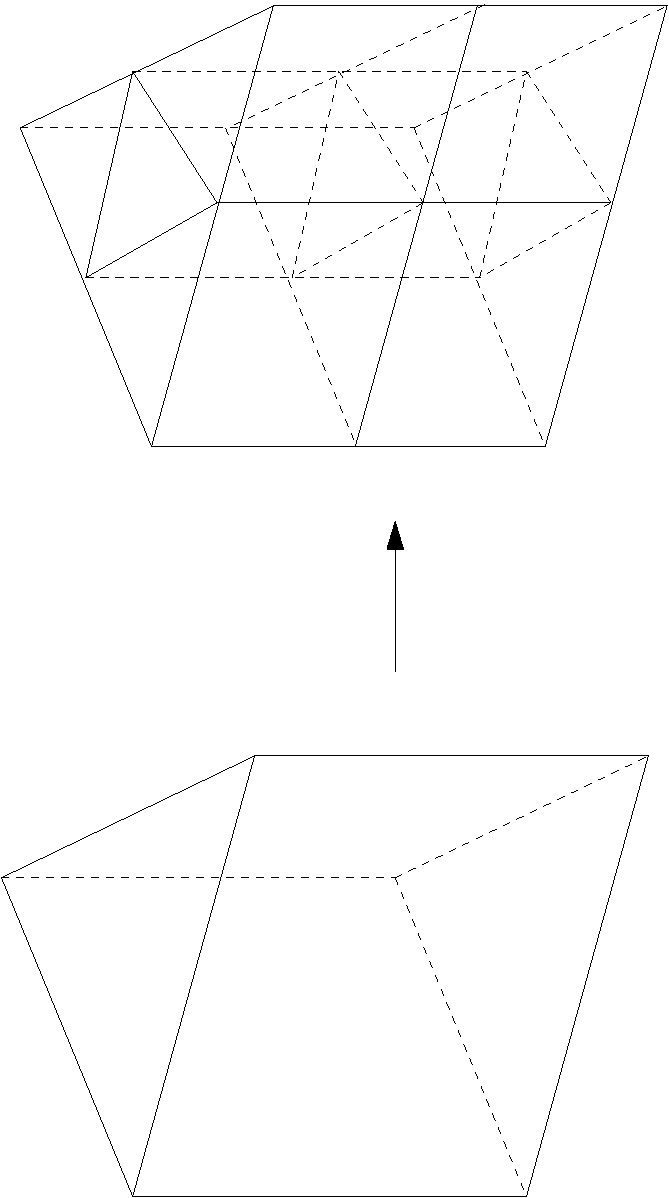
\includegraphics[angle=-90, width=.45\textwidth]{amr/prism_refinement}  \\
    Tetrahedron && Prism
  \end{tabular}
\end{frame}


%%%%%%%%%%%%%%%%%%%%%%%%%%%%%%%%%%%%%%%%%%%%%%%%%%%%%%%%%%%%%%%%%%%%%%%%%%%%%%%
\begin{frame}{Flux-Jump Error Indicator}
\begin{itemize}
\item The flux-jump error indicator is derived starting from the element
  integrals
  % Reference the previously used equation with the same number
    \begin{equation}
      \eqneltint\tag{\ref{eqn:element_integrals}}
    \end{equation}

  \item Applying the divergence theorem ``in reverse'' obtains
    \begin{eqnarray}
      \sum_{e=1}^{N_e} \int_{\Omega_e}
      \left( -\Delta u^h  + (\bv{b} \cdot \nabla u^h) + cu^h
      -f \right) v^h \;  dx + \\
      \nonumber
      \sum_{\partial \Omega_e \not \subset  \partial \Omega}
      \int_{\partial \Omega_e} \left\llbracket \frac{\partial u^h}{\partial n} \right\rrbracket v^h \; dx=0
    \end{eqnarray}
\end{itemize}
\end{frame}


%%%%%%%%%%%%%%%%%%%%%%%%%%%%%%%%%%%%%%%%%%%%%%%%%%%%%%%%%%%%%%%%%%%%%%%%%%%%%%%
\begin{frame}{Flux-Jump Error Indicator (cont.)}
  \begin{itemize}
  \item Defining the cell residual
    \begin{equation}
      r(u^h) = -\Delta u^h  + (\bv{b} \cdot \nabla u^h) + cu^h -f
    \end{equation}
    we have
    \begin{eqnarray}
      \label{eqn:residuals}
      \sum_{e=1}^{N_e} \int_{\Omega_e}
      r(u^h) v^h \;  dx +
      \sum_{\partial \Omega_e \not \subset  \partial \Omega}
      \int_{\partial \Omega_e} \left\llbracket \frac{\partial u^h}{\partial n} \right\rrbracket v^h \; dx=0
    \end{eqnarray}

  \item Clearly, the exact solution $u$ satisfies~\eqref{eqn:residuals} identically.

  \item Computing $r(u^h)$ requires
    knowledge of the differential operator (i.e.\ knowledge of the ``physics'').

  \item The second sum leads to a \emph{physics-independent} method for estimating the
    error in the approximate solution $u^h$.

  \end{itemize}
\end{frame}



%%%%%%%%%%%%%%%%%%%%%%%%%%%%%%%%%%%%%%%%%%%%%%%%%%%%%%%%%%%%%%%%%%%%%%%%%%%%%%%
\begin{frame}{Flux-Jump Error Indicator (cont.)}
\begin{itemize}
  \item Pros
    \begin{itemize}
      \item Ideal for low-order (piecewise linear) elements
      \item Easily extensible to adaptivity with hanging nodes
      \item Works well in practice for nonlinear, time-dependent problems,
	and problems with shocks, layers, discontinuities, etc.
    \end{itemize}

  \item Cons
    \begin{itemize}
    \item For higher-order elements, the interior residual term may dominate
    \item Relatively expensive to compute
    \item Makes no sense for discontinuous and $C^1$ FE bases
    \end{itemize}
\end{itemize}

\end{frame}



%%%%%%%%%%%%%%%%%%%%%%%%%%%%%%%%%%%%%%%%%%%%%%%%%%%%%%%%%%%%%%%%%%%%%%%%%%%%%%%
\begin{frame}{1D Example}
\begin{itemize}
\item In 1 dimension, the jump integrals reduce to point-wise evaluation
  of the derivatives at the element boundaries.

  \item For linear elements, the error indicator $\eta$ for a particular element
    $\Omega_e = (x_e, x_{e+1})$ is defined as
    \begin{equation}
      \eta^2 =
      %\left\{
      %\begin{array}{c}
%	h_e \llbracket u'(x_2) \rrbracket^2 \\
      %\frac{h_e}{2} \left( \llbracket u'(x_e) \rrbracket^2 + \llbracket u'(x_{e+1}) \rrbracket^2 \right) \\
%	h_e \llbracket u'(x_{N_e}) \rrbracket^2
 %     \end{array}
 %     \right.
	\frac{h_e}{N_{\text{int}}} \sum_{i=1}^{N_{\text{int}}}  \llbracket u'(y_i) \rrbracket^2
    \end{equation}
    where $h_e = x_{e+1} - x_e$ is the element length, and $N_{\text{int}} \leq 2$ is the number of
    \emph{interior} nodes $y_i$ the element has.

%  \item The flux-jump indicator for elements on Dirichlet boundaries weights the jump
%    at the single interior node twice.
\end{itemize}

\end{frame}



%%%%%%%%%%%%%%%%%%%%%%%%%%%%%%%%%%%%%%%%%%%%%%%%%%%%%%%%%%%%%%%%%%%%%%%%%%%%%%%
\begin{frame}{1D Example (cont.)}
  \begin{columns}
    \column{.65\textwidth}
    \begin{itemize}
    \item Consider the function
      \begin{equation}
        \nonumber
        u = \frac{1-\exp(10x)}{1-\exp(10)}
      \end{equation}
      which is a solution of the classic 1D advection-diffusion boundary layer equation.
\item We assume here that the finite element solution is the linear
  interpolant of $u$, and compute the error indicator for a sequence of
  uniformly refined grids.
\end{itemize}

      \column{.35\textwidth}
  \begin{center}
    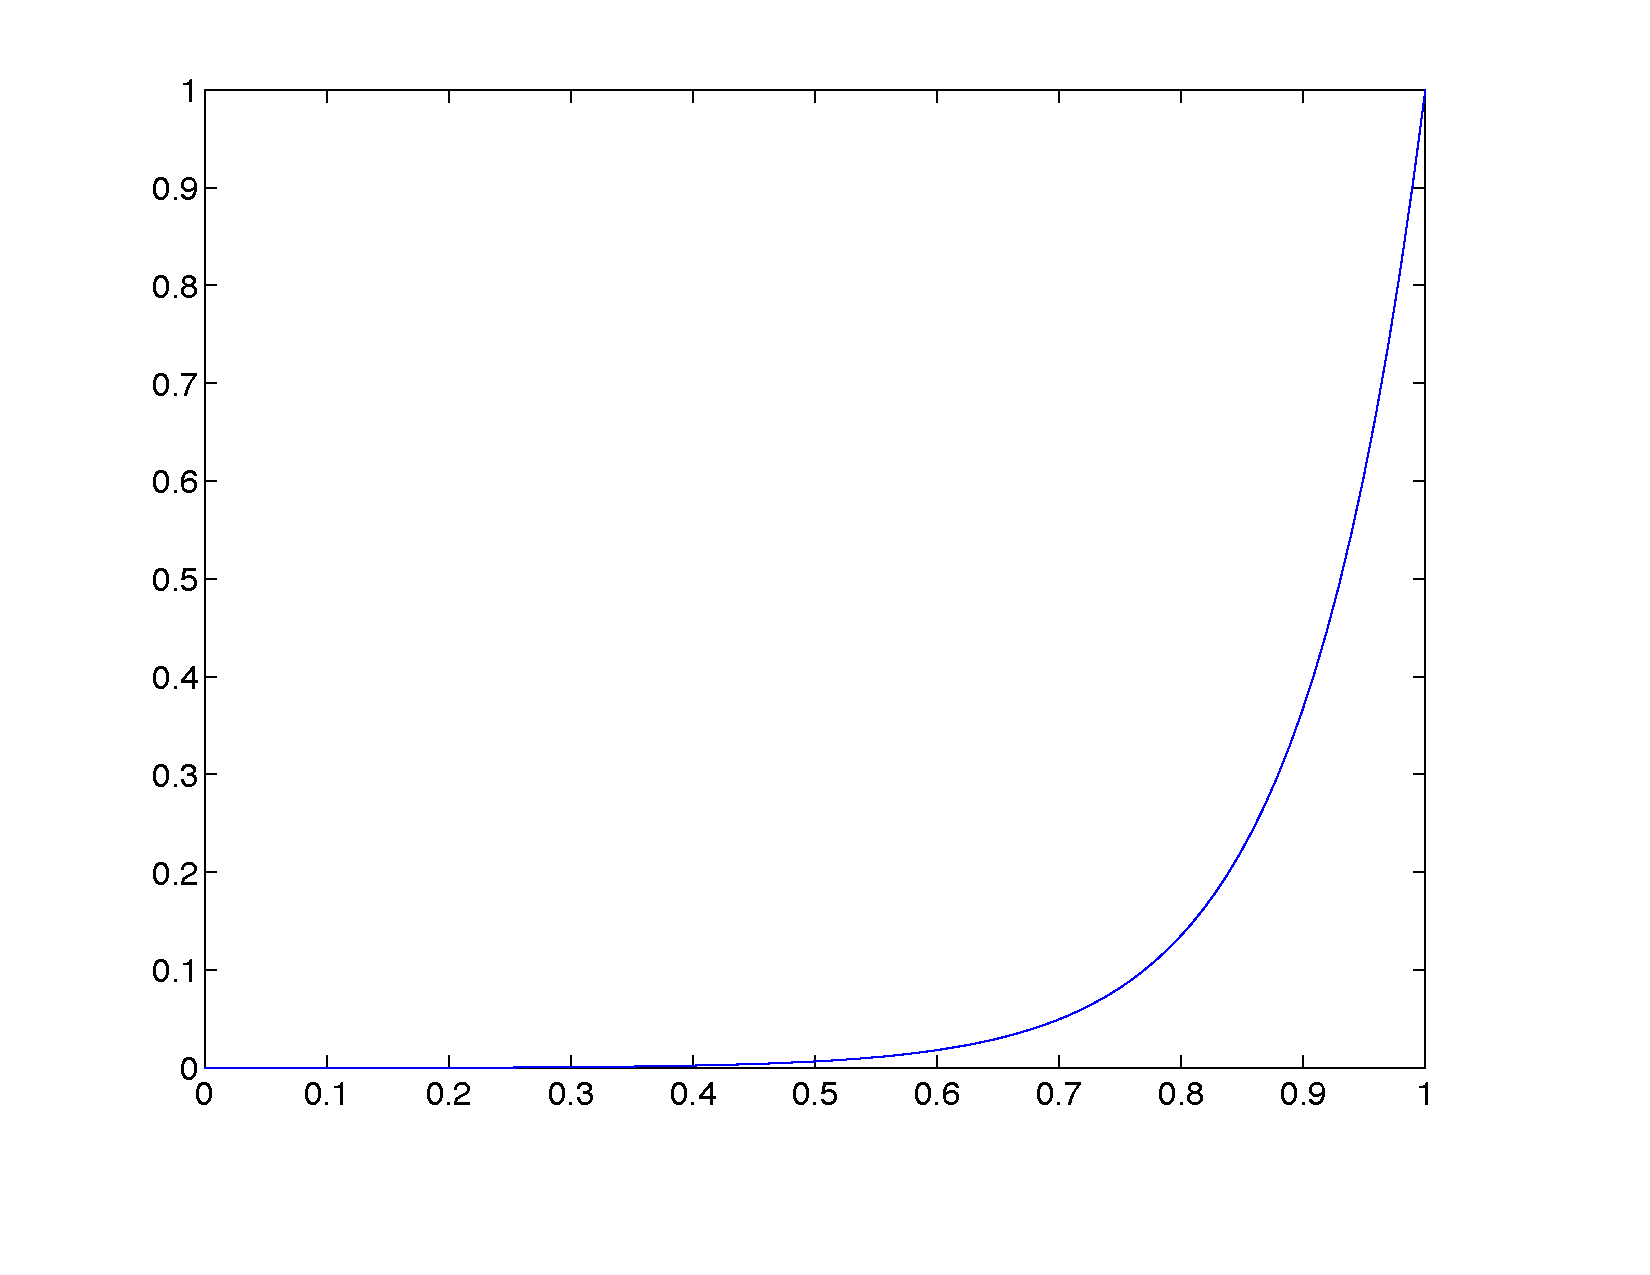
\includegraphics[viewport=50 50 700 600,width=.9\textwidth]{amr/bl}
  \end{center}
  \end{columns}
\end{frame}



%%%%%%%%%%%%%%%%%%%%%%%%%%%%%%%%%%%%%%%%%%%%%%%%%%%%%%%%%%%%%%%%%%%%%%%%%%%%%%%
\begin{frame}%{1D Example (cont.)}
  \only<1>
  {
    \begin{tabular}{cc} \\
      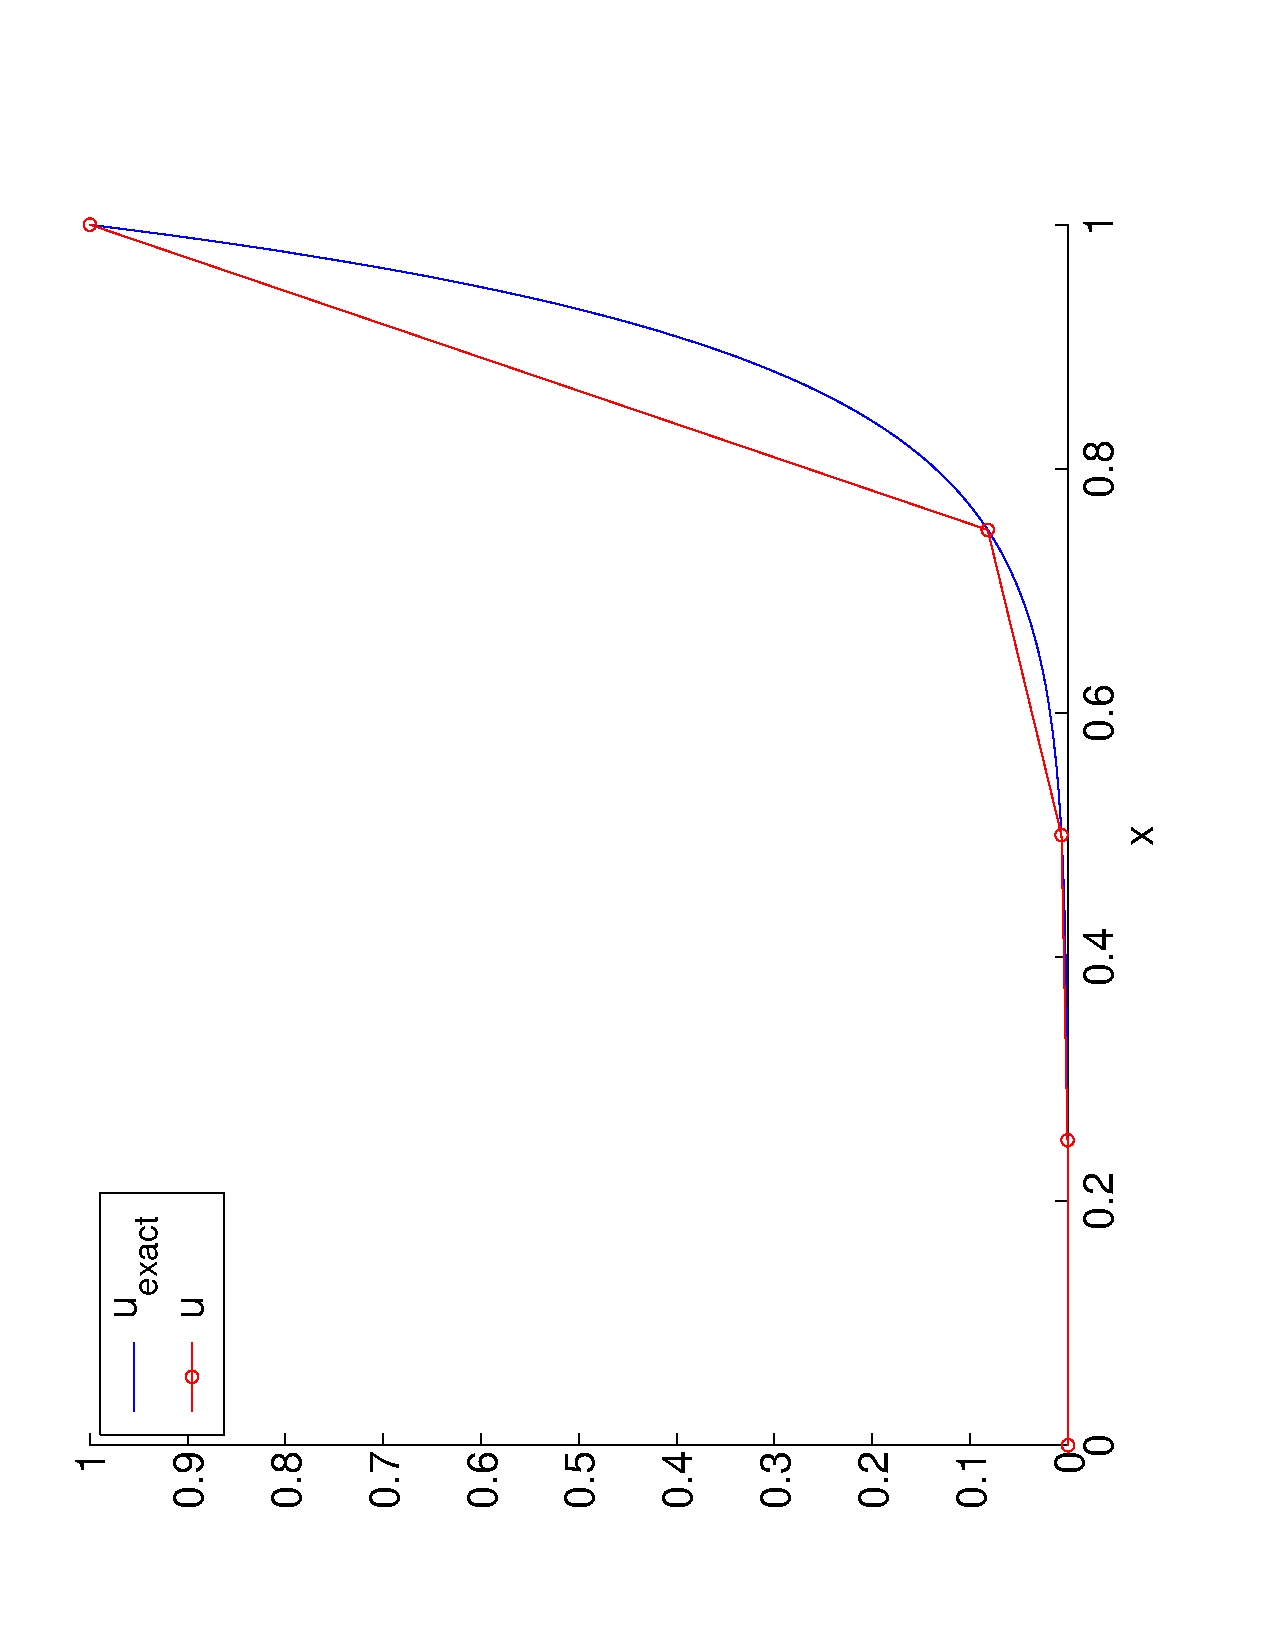
\includegraphics[angle=-90,width=.42\textwidth]{amr/u_bl_5elems}&
      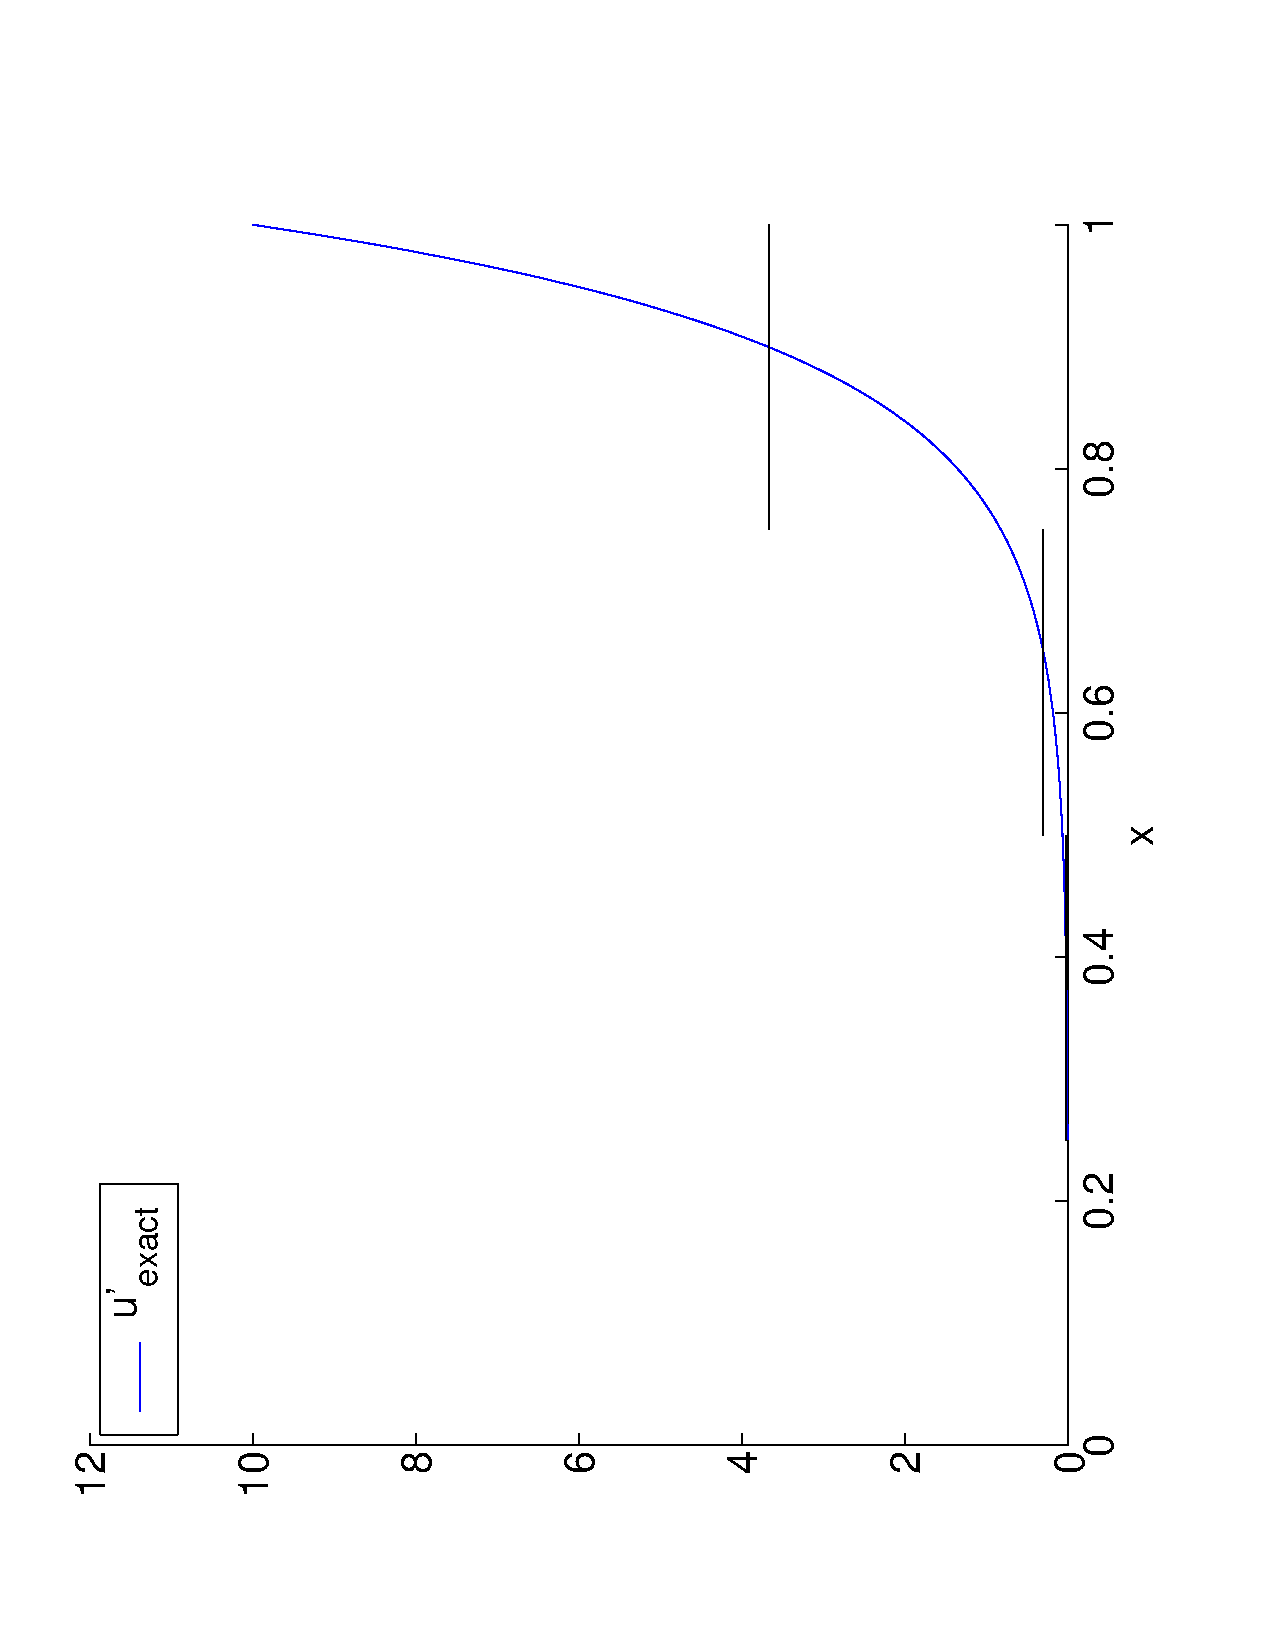
\includegraphics[angle=-90,width=.42\textwidth]{amr/up_bl_5elems} \\
      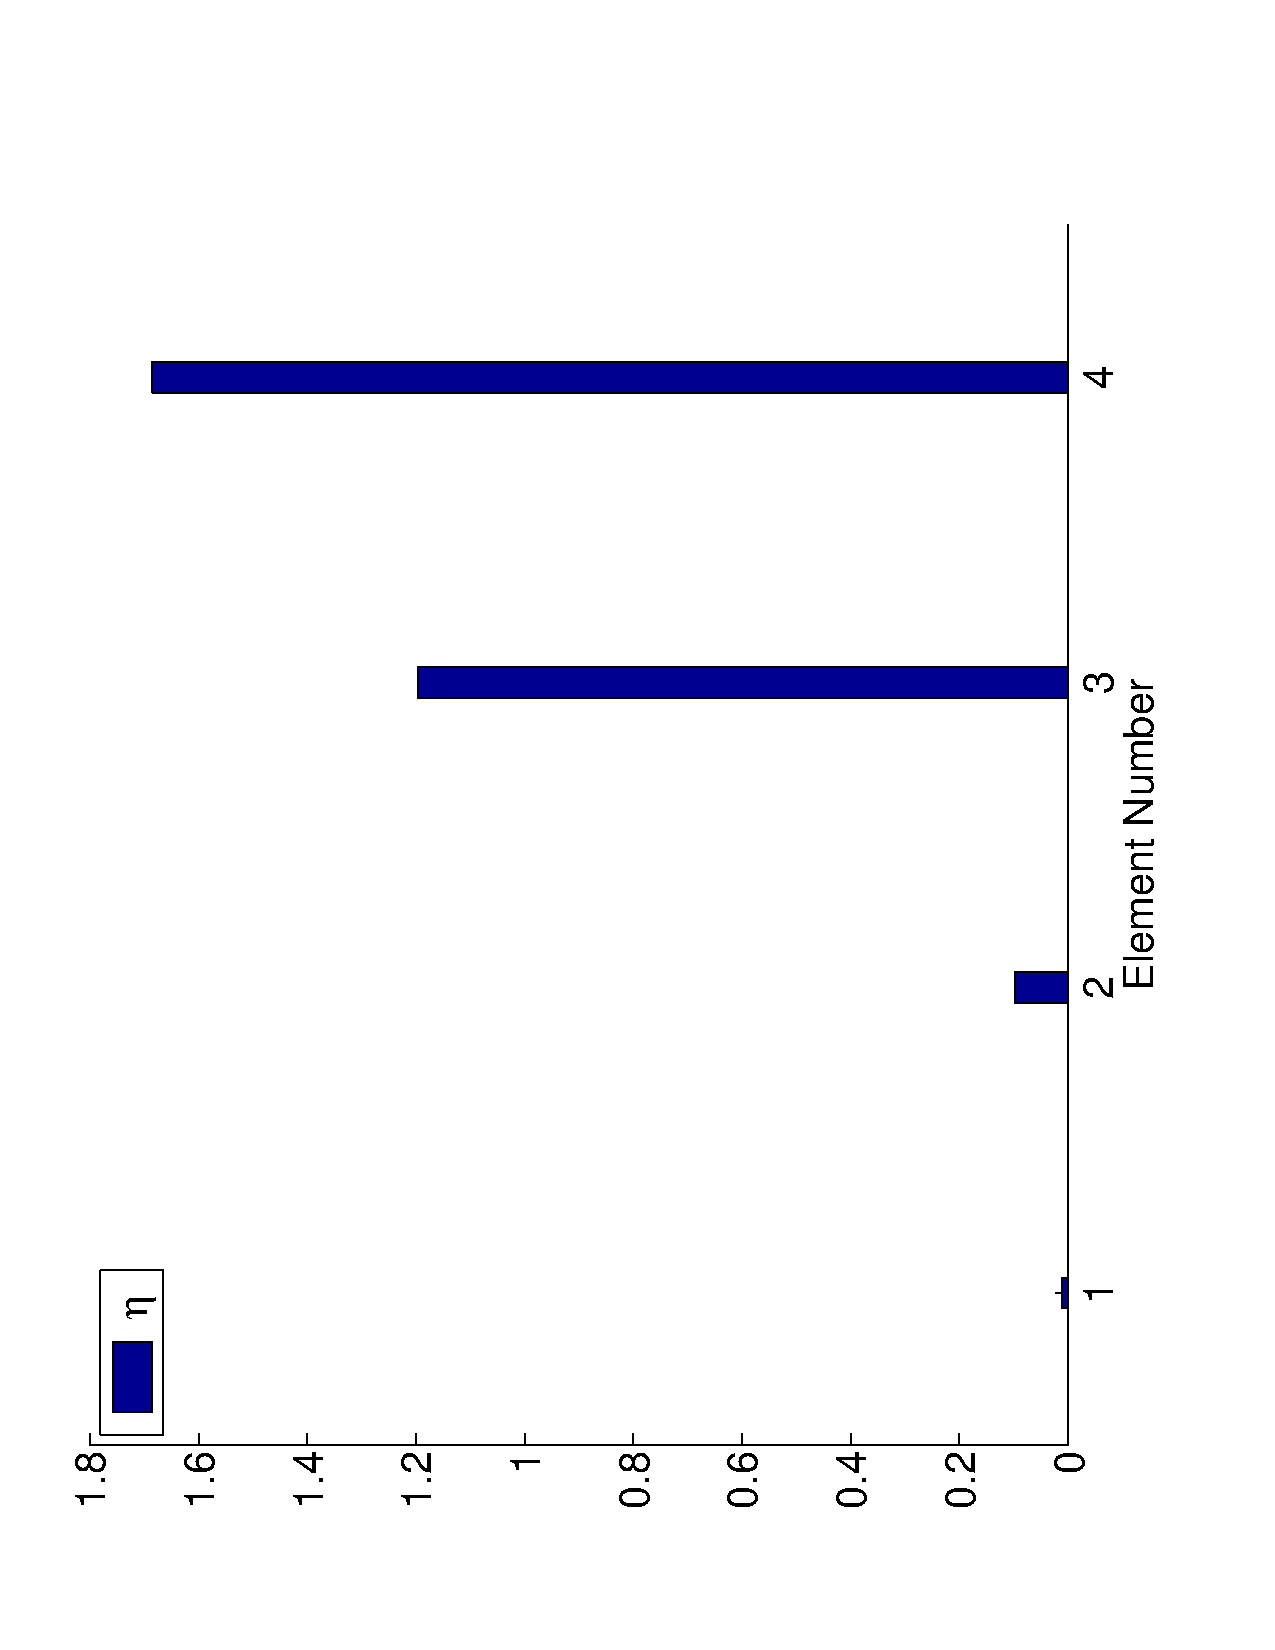
\includegraphics[angle=-90,width=.42\textwidth]{amr/eta_bl_5elems}&
      $\begin{array}{c}
        \text{4 elements} \\
        ||e||_{L_2} = 0.09
      \end{array}$\\
    \end{tabular}
  }
  \only<2>
  {
    \begin{tabular}{cc} \\
      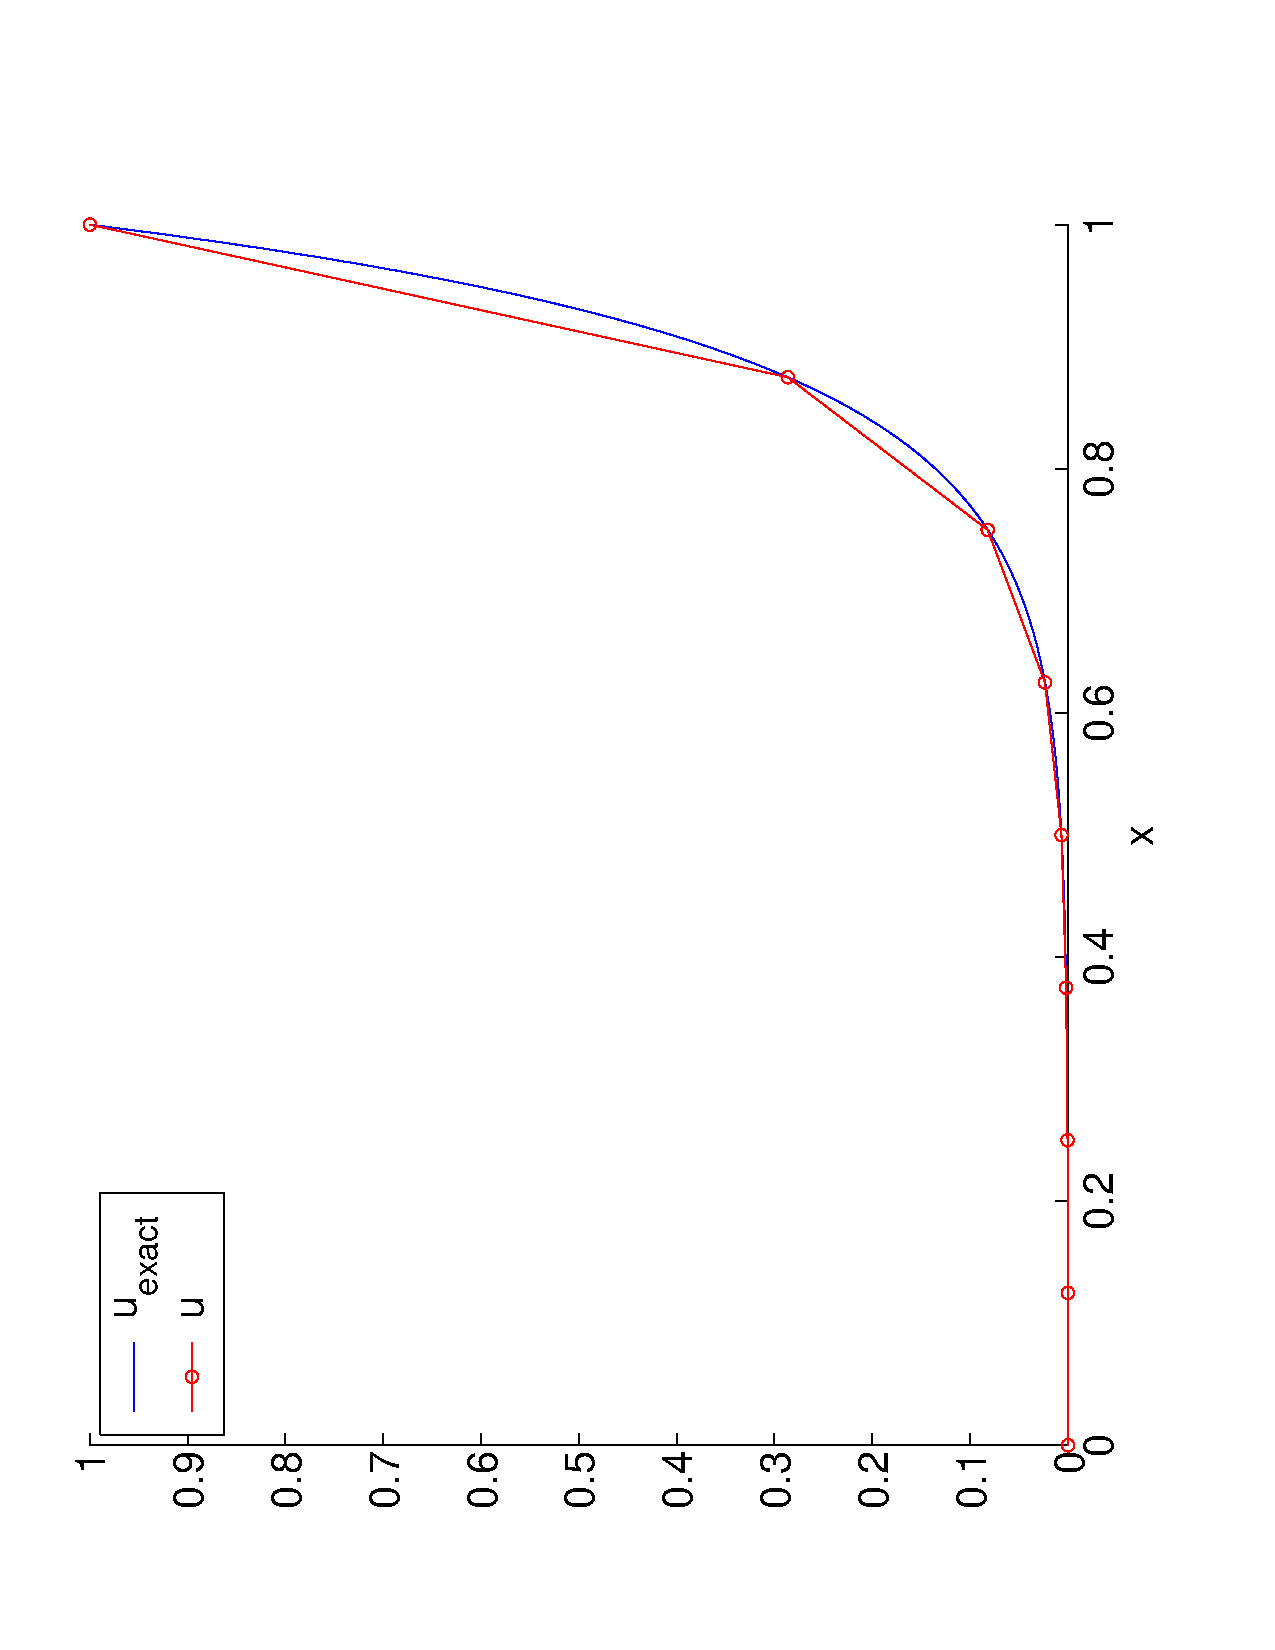
\includegraphics[angle=-90,width=.42\textwidth]{amr/u_bl_9elems}&
      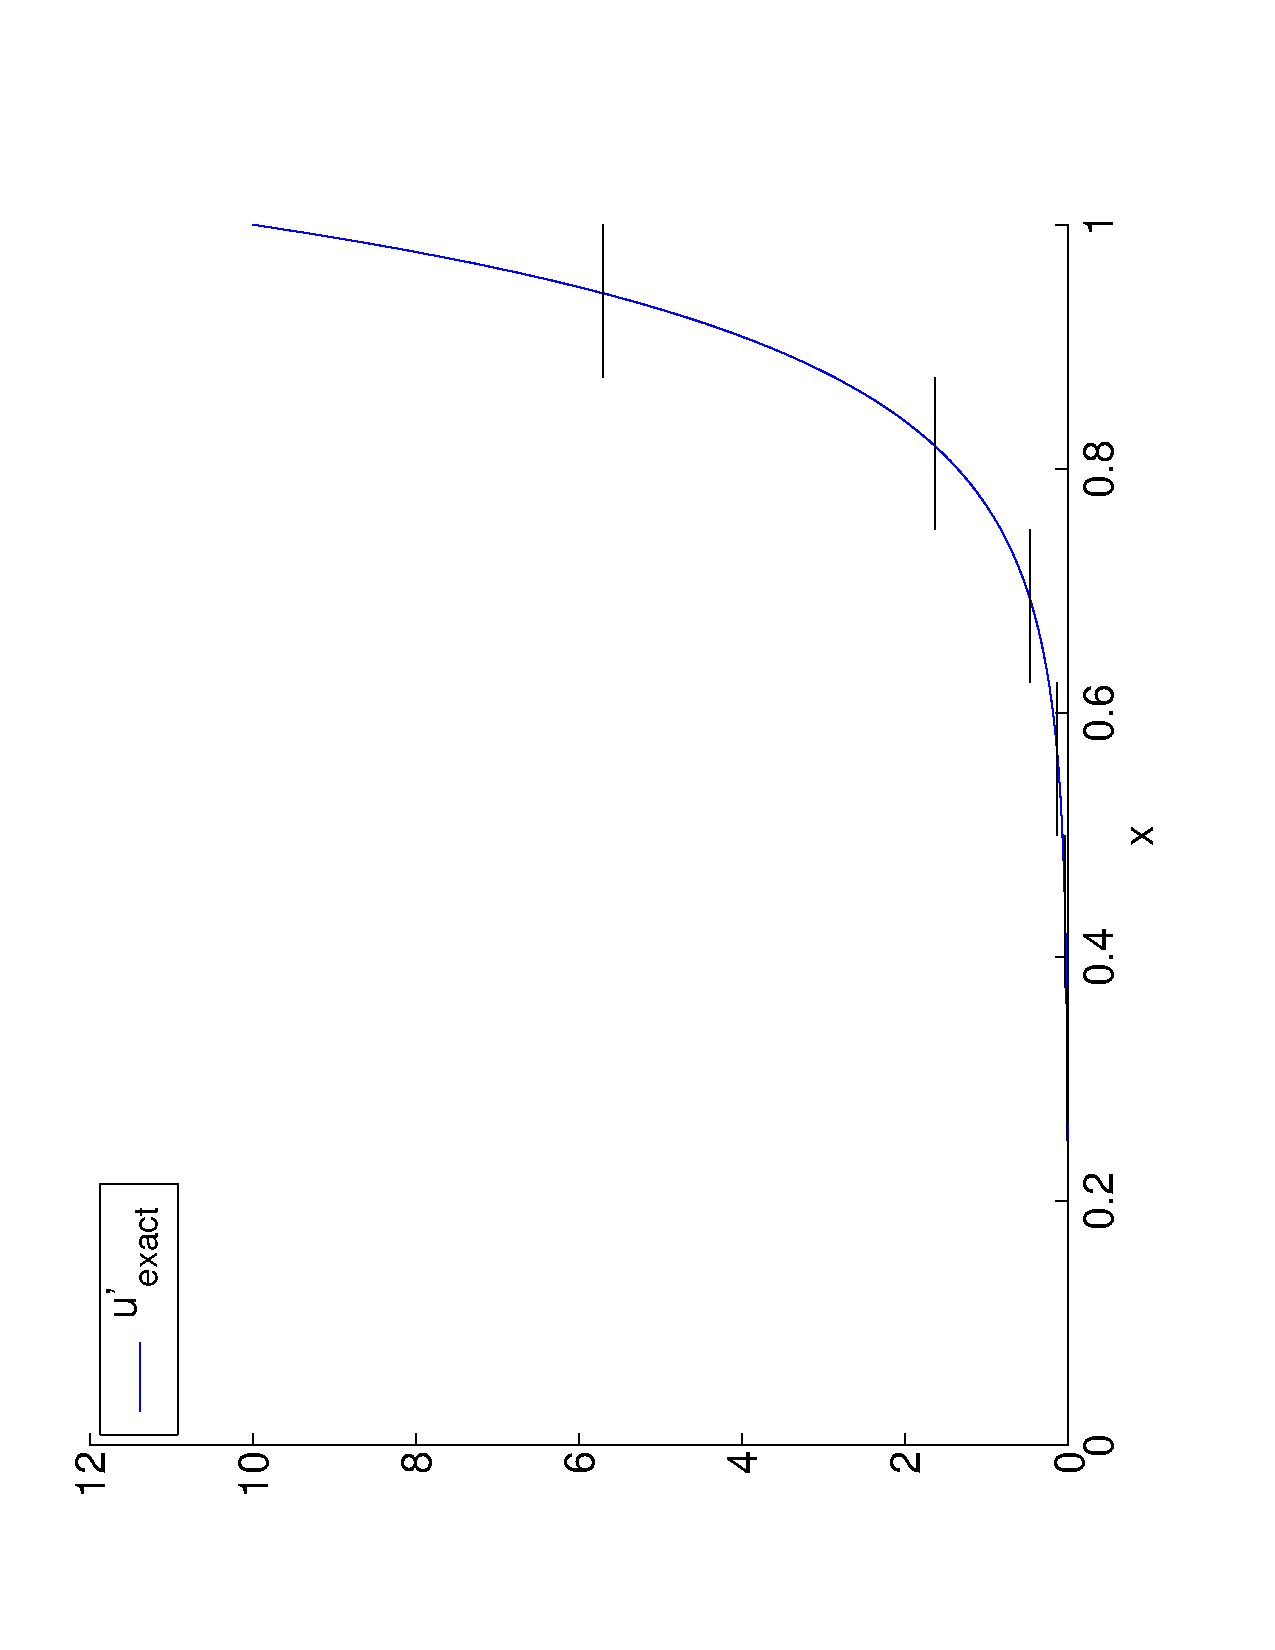
\includegraphics[angle=-90,width=.42\textwidth]{amr/up_bl_9elems} \\
      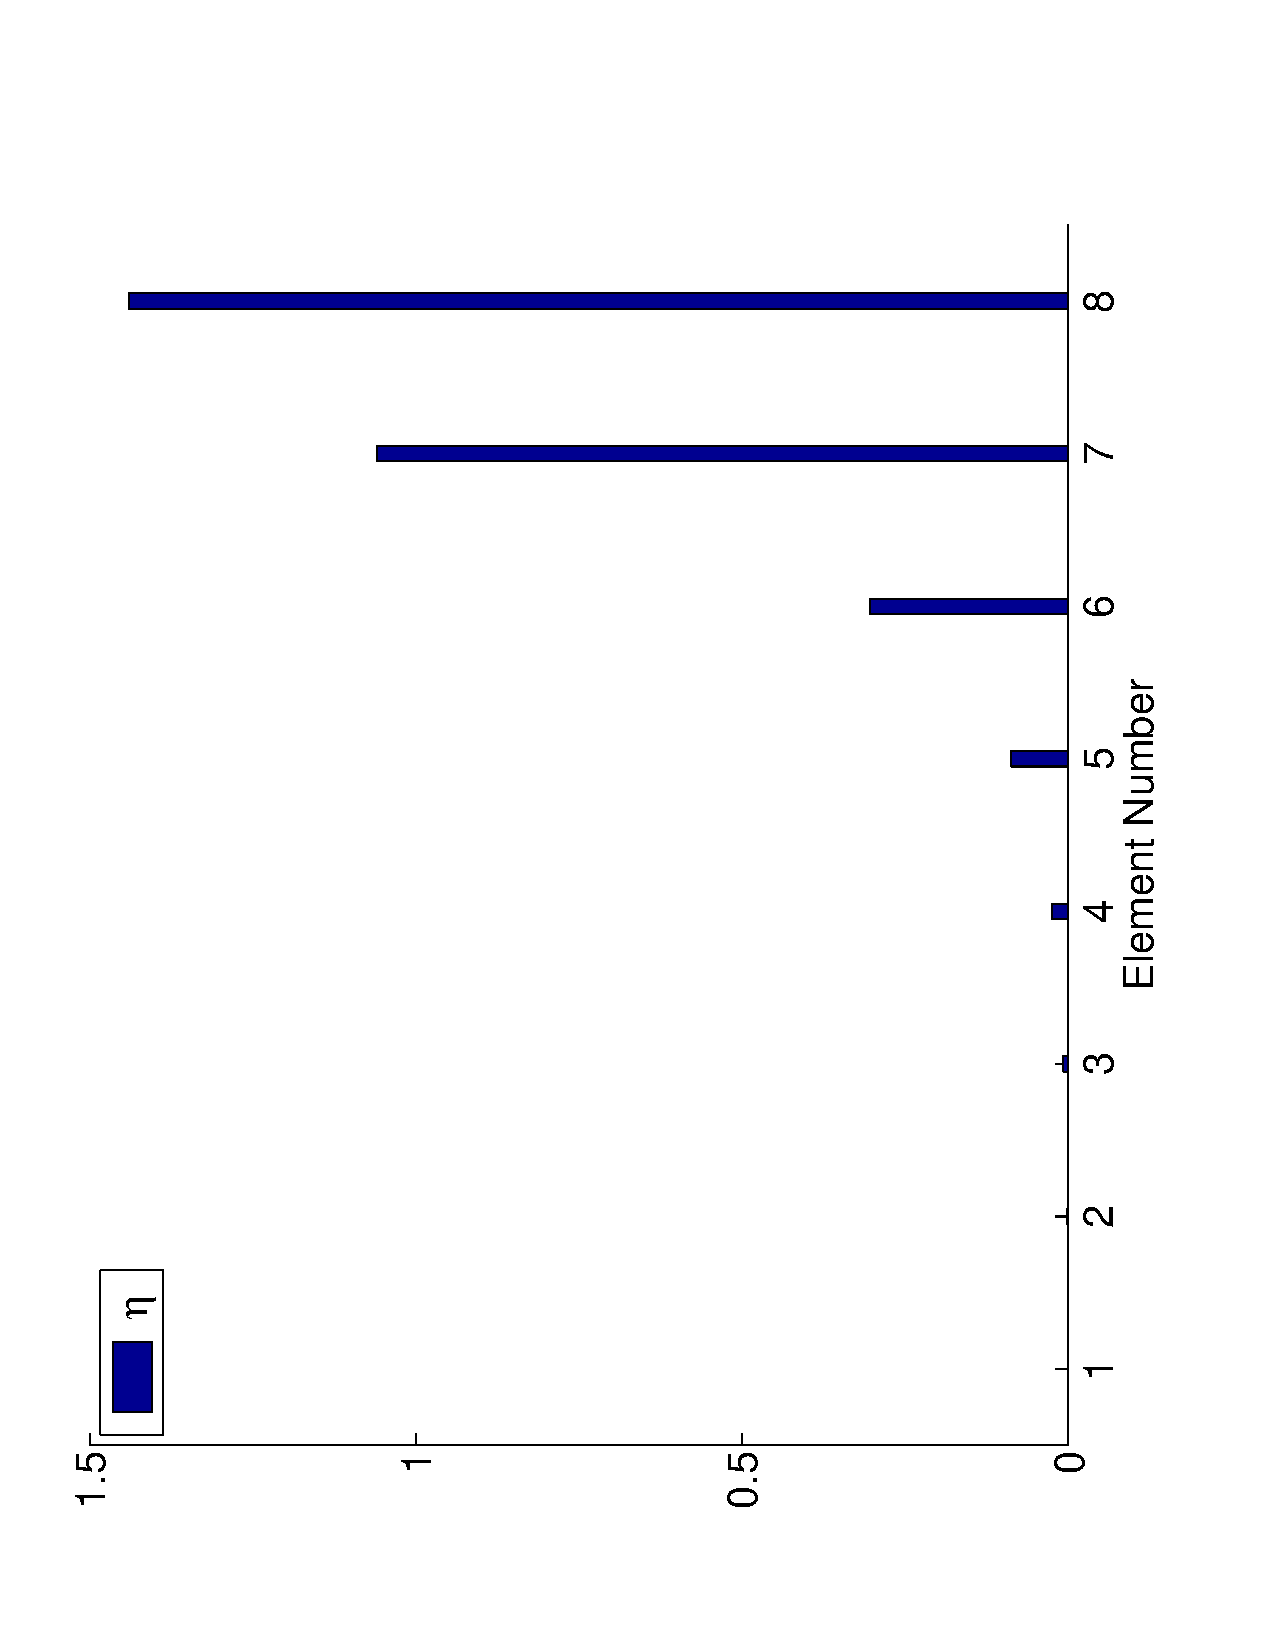
\includegraphics[angle=-90,width=.42\textwidth]{amr/eta_bl_9elems}&
      $\begin{array}{c}
        \text{8 elements} \\
        ||e||_{L_2} = 0.027
      \end{array}$\\
    \end{tabular}
  }
  \only<3>
  {
    \begin{tabular}{cc} \\
      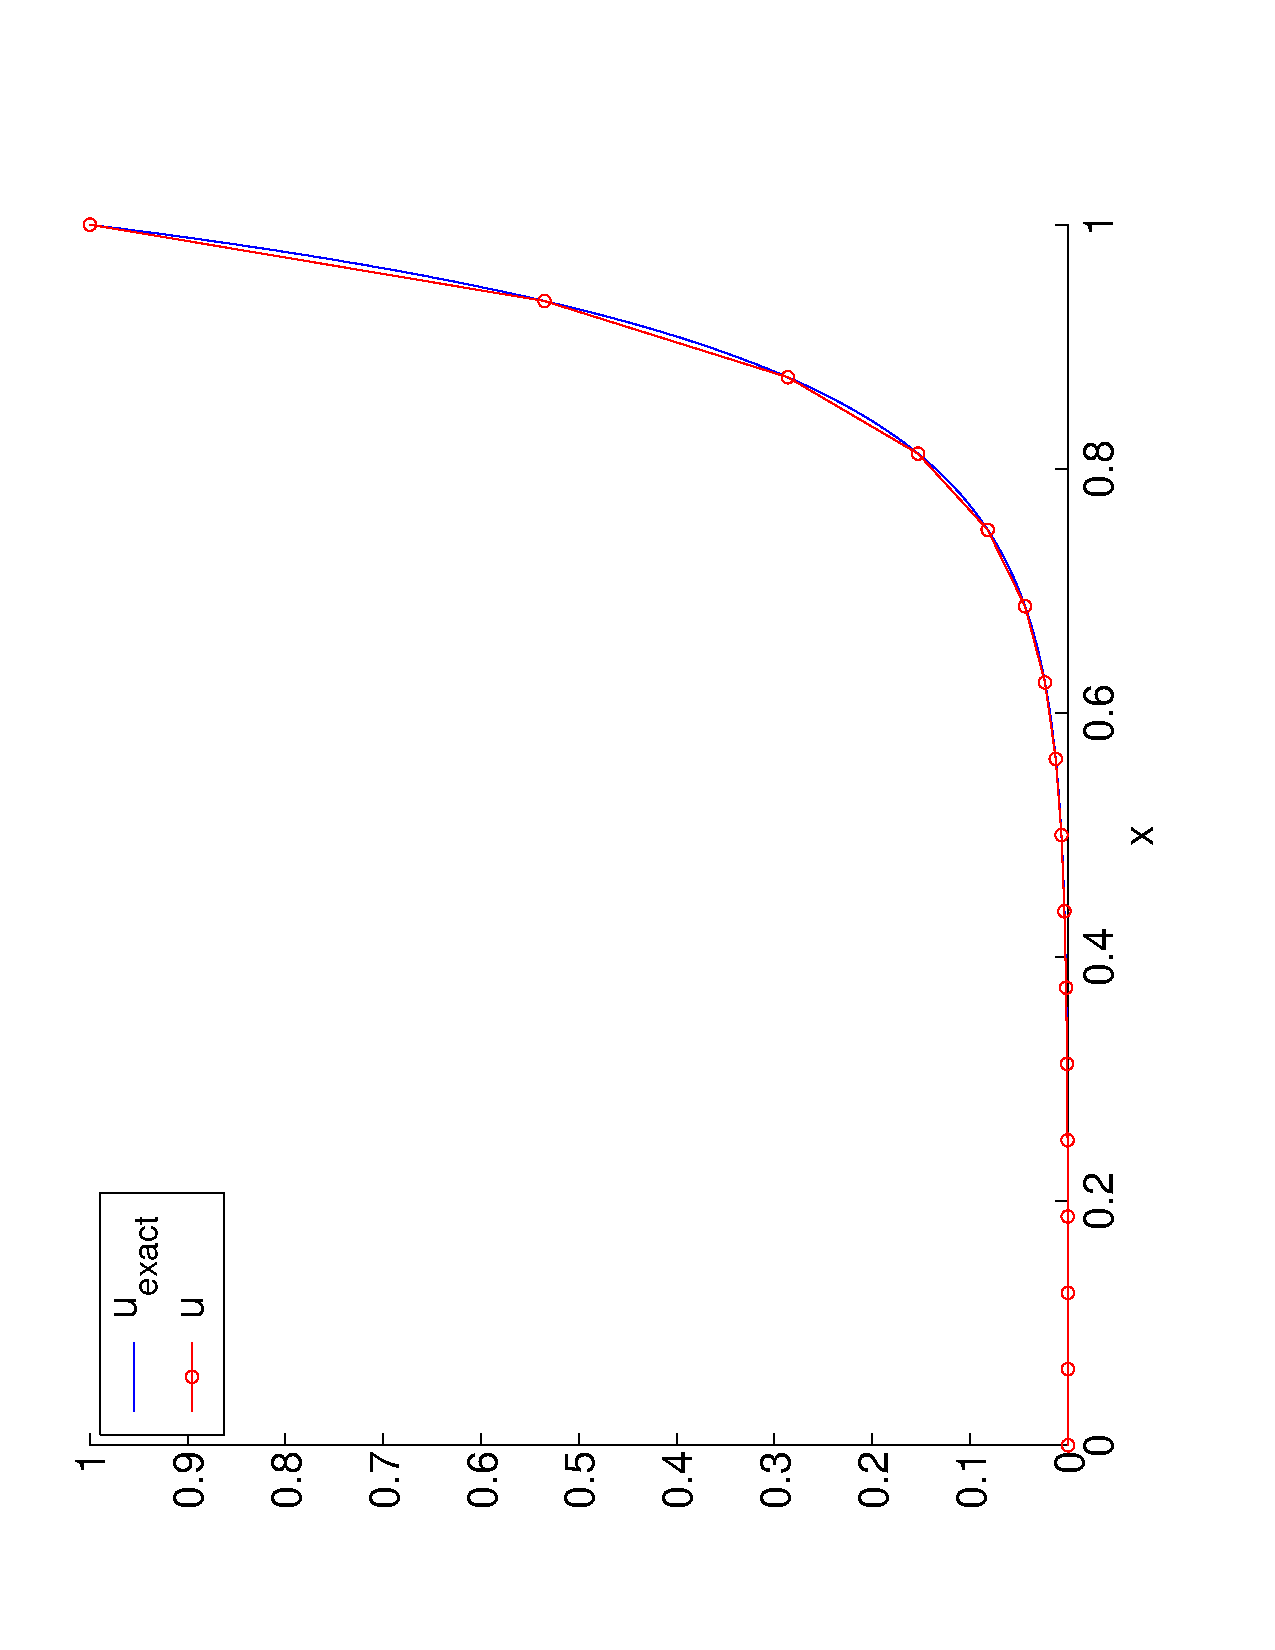
\includegraphics[angle=-90,width=.42\textwidth]{amr/u_bl_17elems}&
      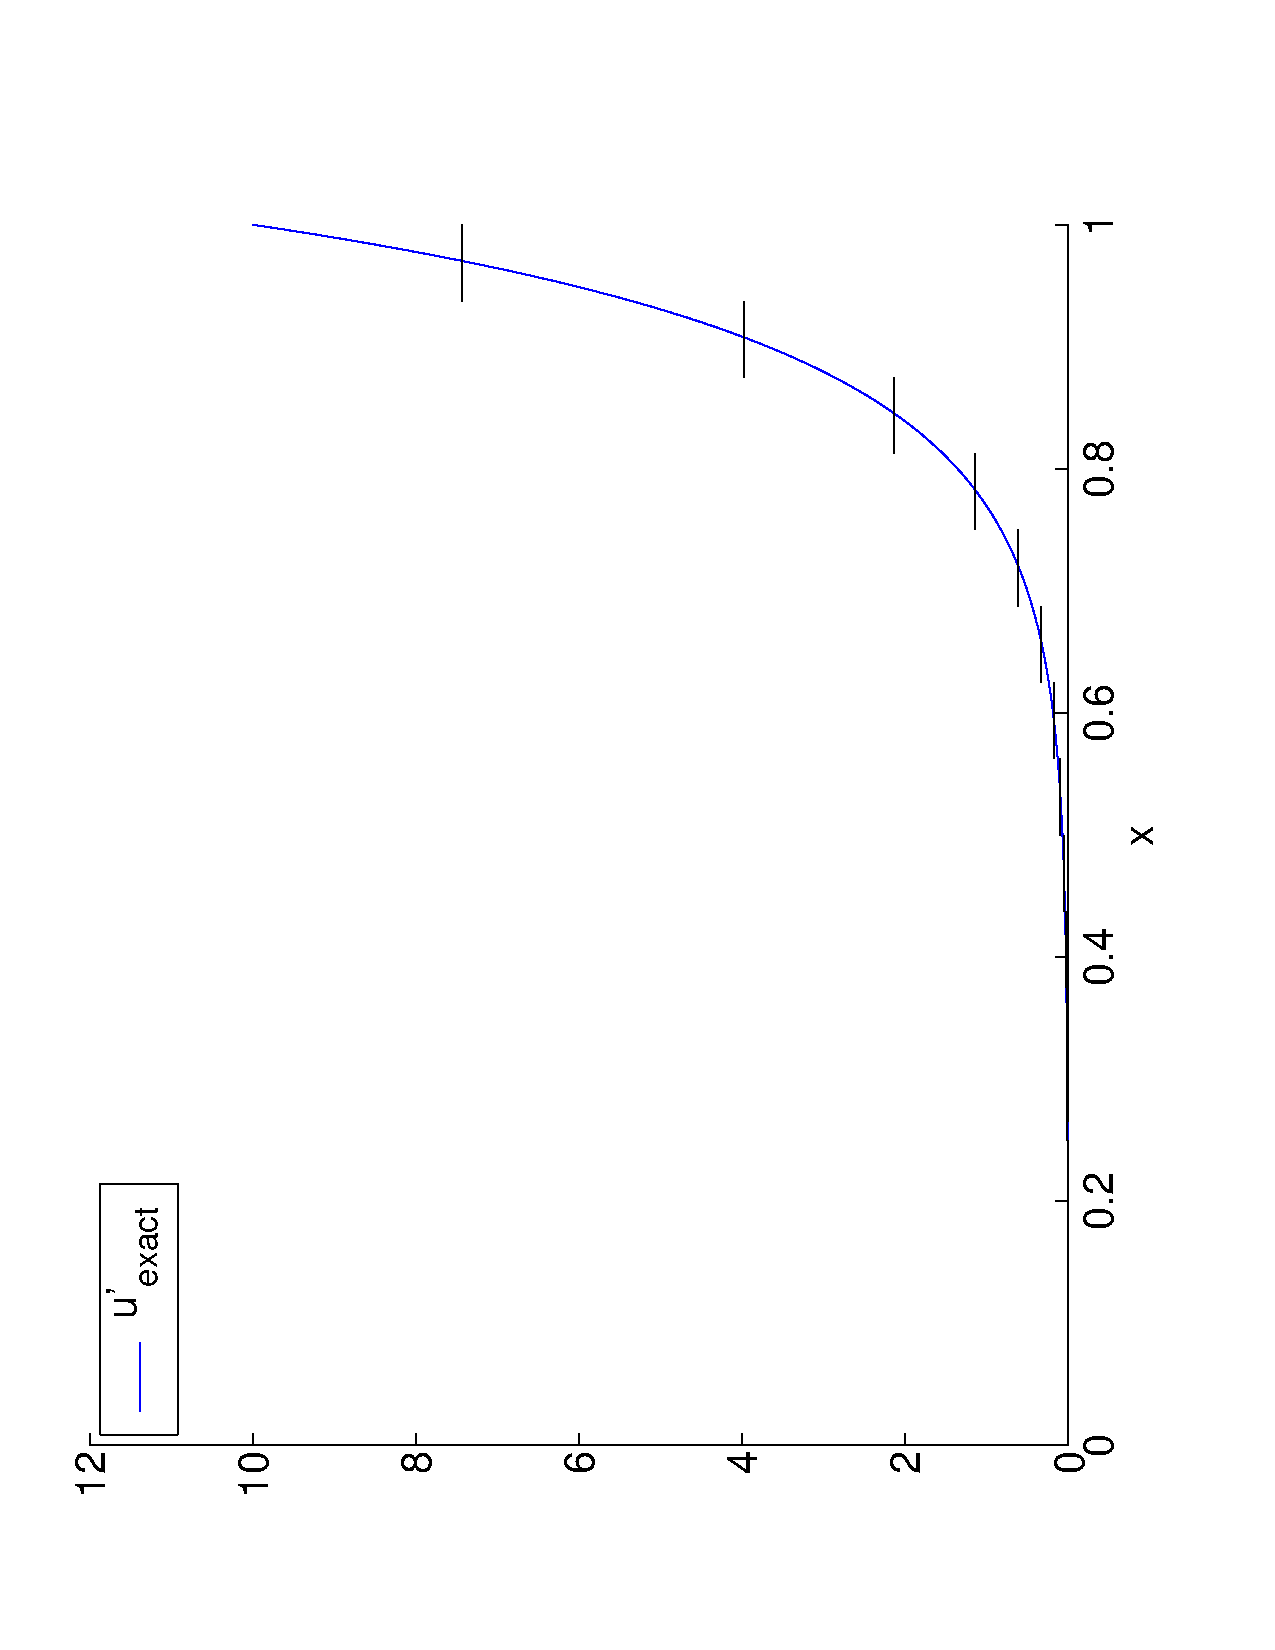
\includegraphics[angle=-90,width=.42\textwidth]{amr/up_bl_17elems} \\
      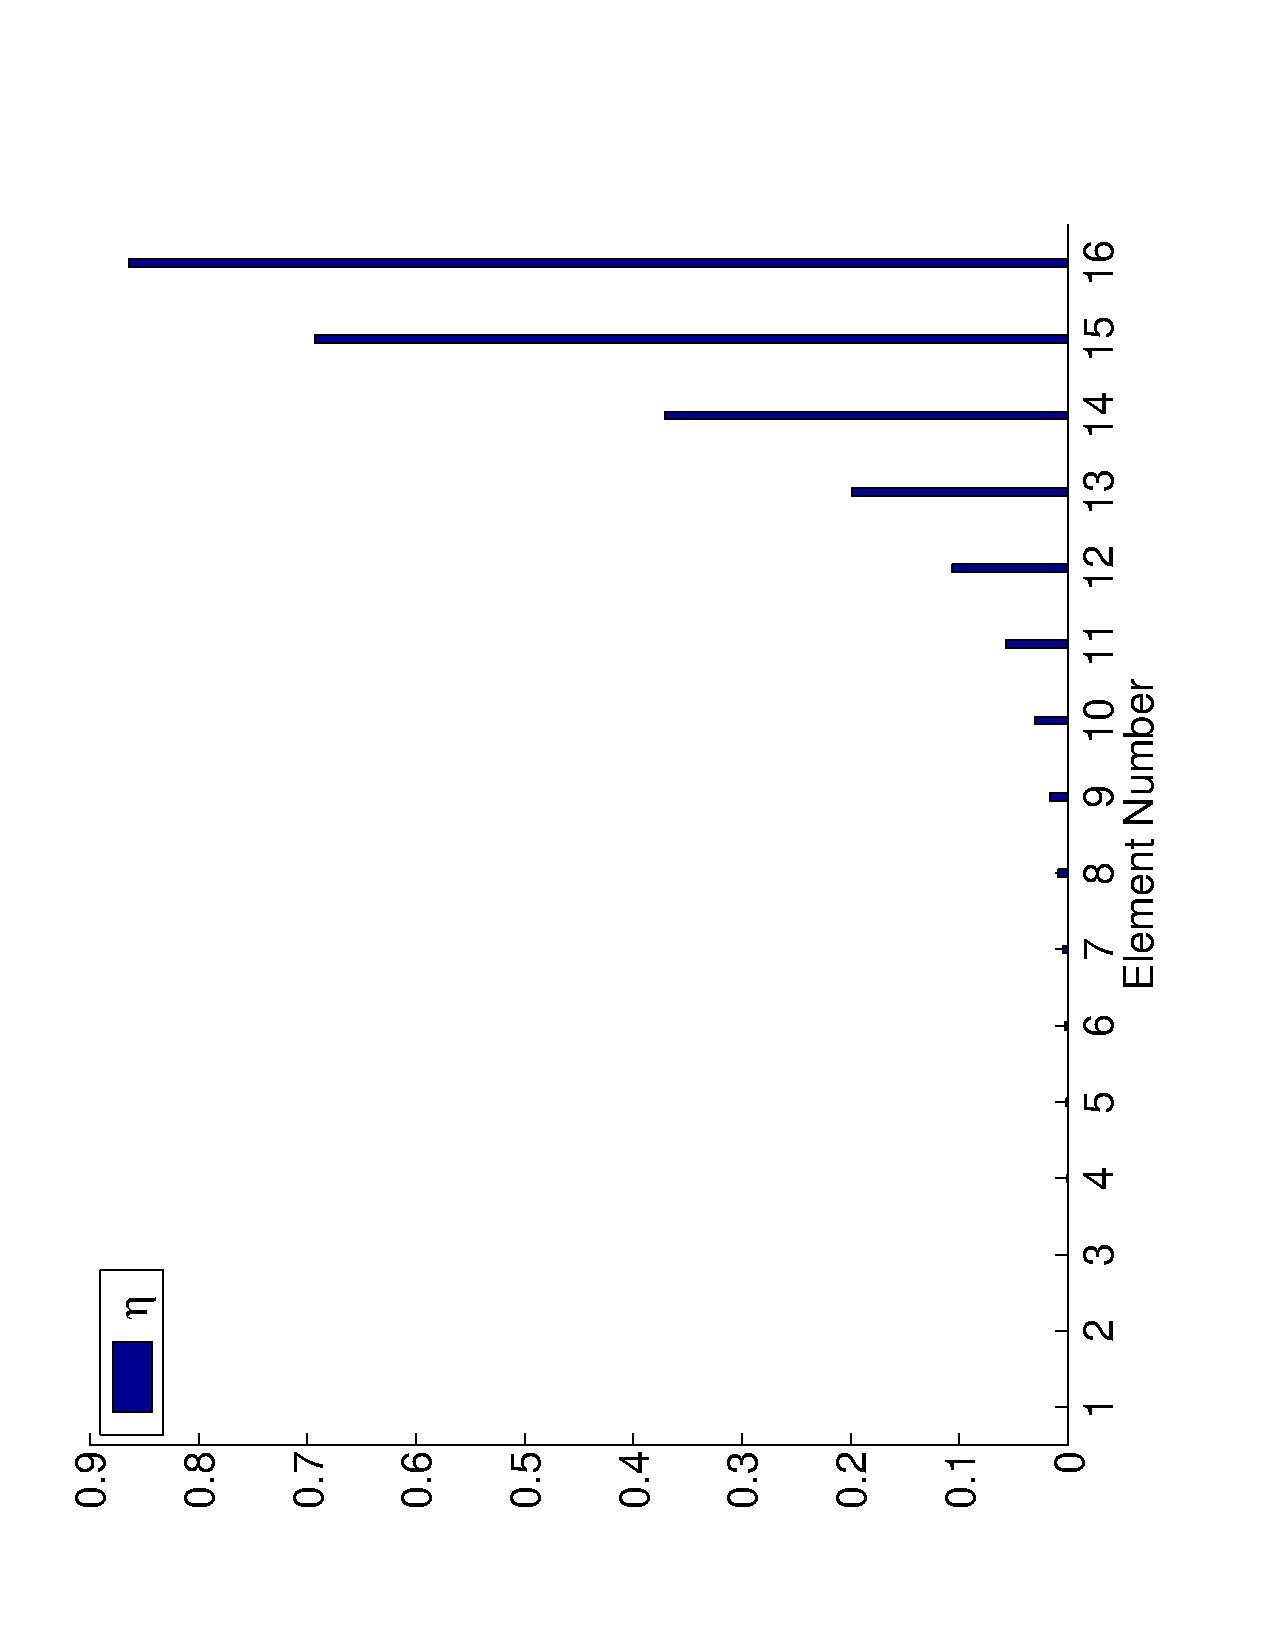
\includegraphics[angle=-90,width=.42\textwidth]{amr/eta_bl_17elems}&
      $\begin{array}{c}
        \text{16 elements} \\
        ||e||_{L_2} = 0.0071
      \end{array}$\\
    \end{tabular}
  }
\end{frame}



%%%%%%%%%%%%%%%%%%%%%%%%%%%%%%%%%%%%%%%%%%%%%%%%%%%%%%%%%%%%%%%%%%%%%%%%%%%%%%%
\begin{frame}[fragile]{A Simple Refinement Strategy}

  \begin{itemize}
    \item A simple adaptive refinement strategy with \texttt{r\_max} refinement steps
      for this 1D example problem is:
  \end{itemize}

%%   \begin{enumerate}
%%   \item Determine an initial grid (e.g. two elements)
%%   \item Compute the FE solution (linear interpolant)
%%   \item Estimate the error in the FE solution using the flux-jump indicator
%%   \item Refine (by splitting) the elements whose error is in the top 10\%
%%   \item Return to step 2.
%%   \end{enumerate}

\small
\begin{semiverbatim}
r=0;
while (r < r_max)
  Compute the FE solution (linear interpolant)
  Estimate the error (using flux-jump indicator)
  Refine the elements with error in top 10\%
  Increment r
end
\end{semiverbatim}
\end{frame}


%%%%%%%%%%%%%%%%%%%%%%%%%%%%%%%%%%%%%%%%%%%%%%%%%%%%%%%%%%%%%%%%%%%%%%%%%%%%%%%
\begin{frame}
  \only<1> {  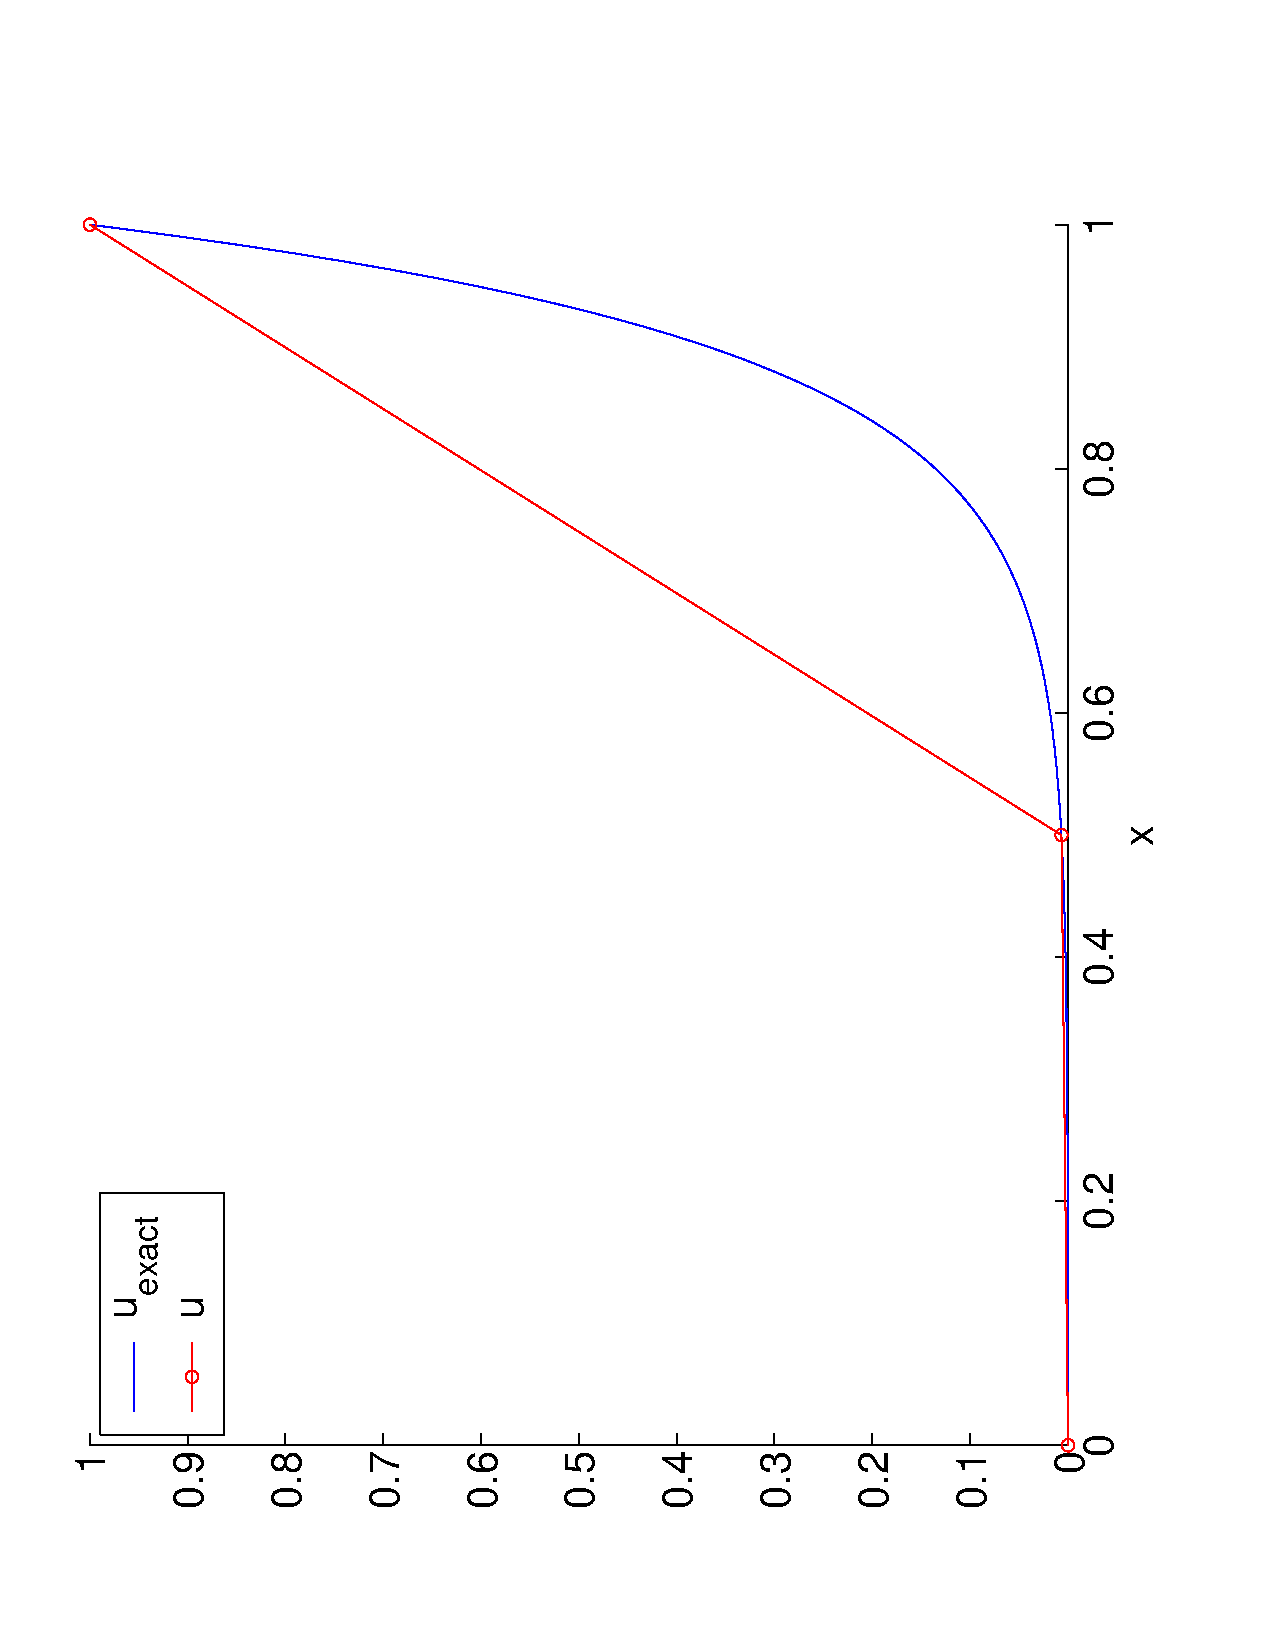
\includegraphics[width=.7\textwidth,angle=-90]{amr/adaptive_u_bl_2elems} }
  \only<2> {  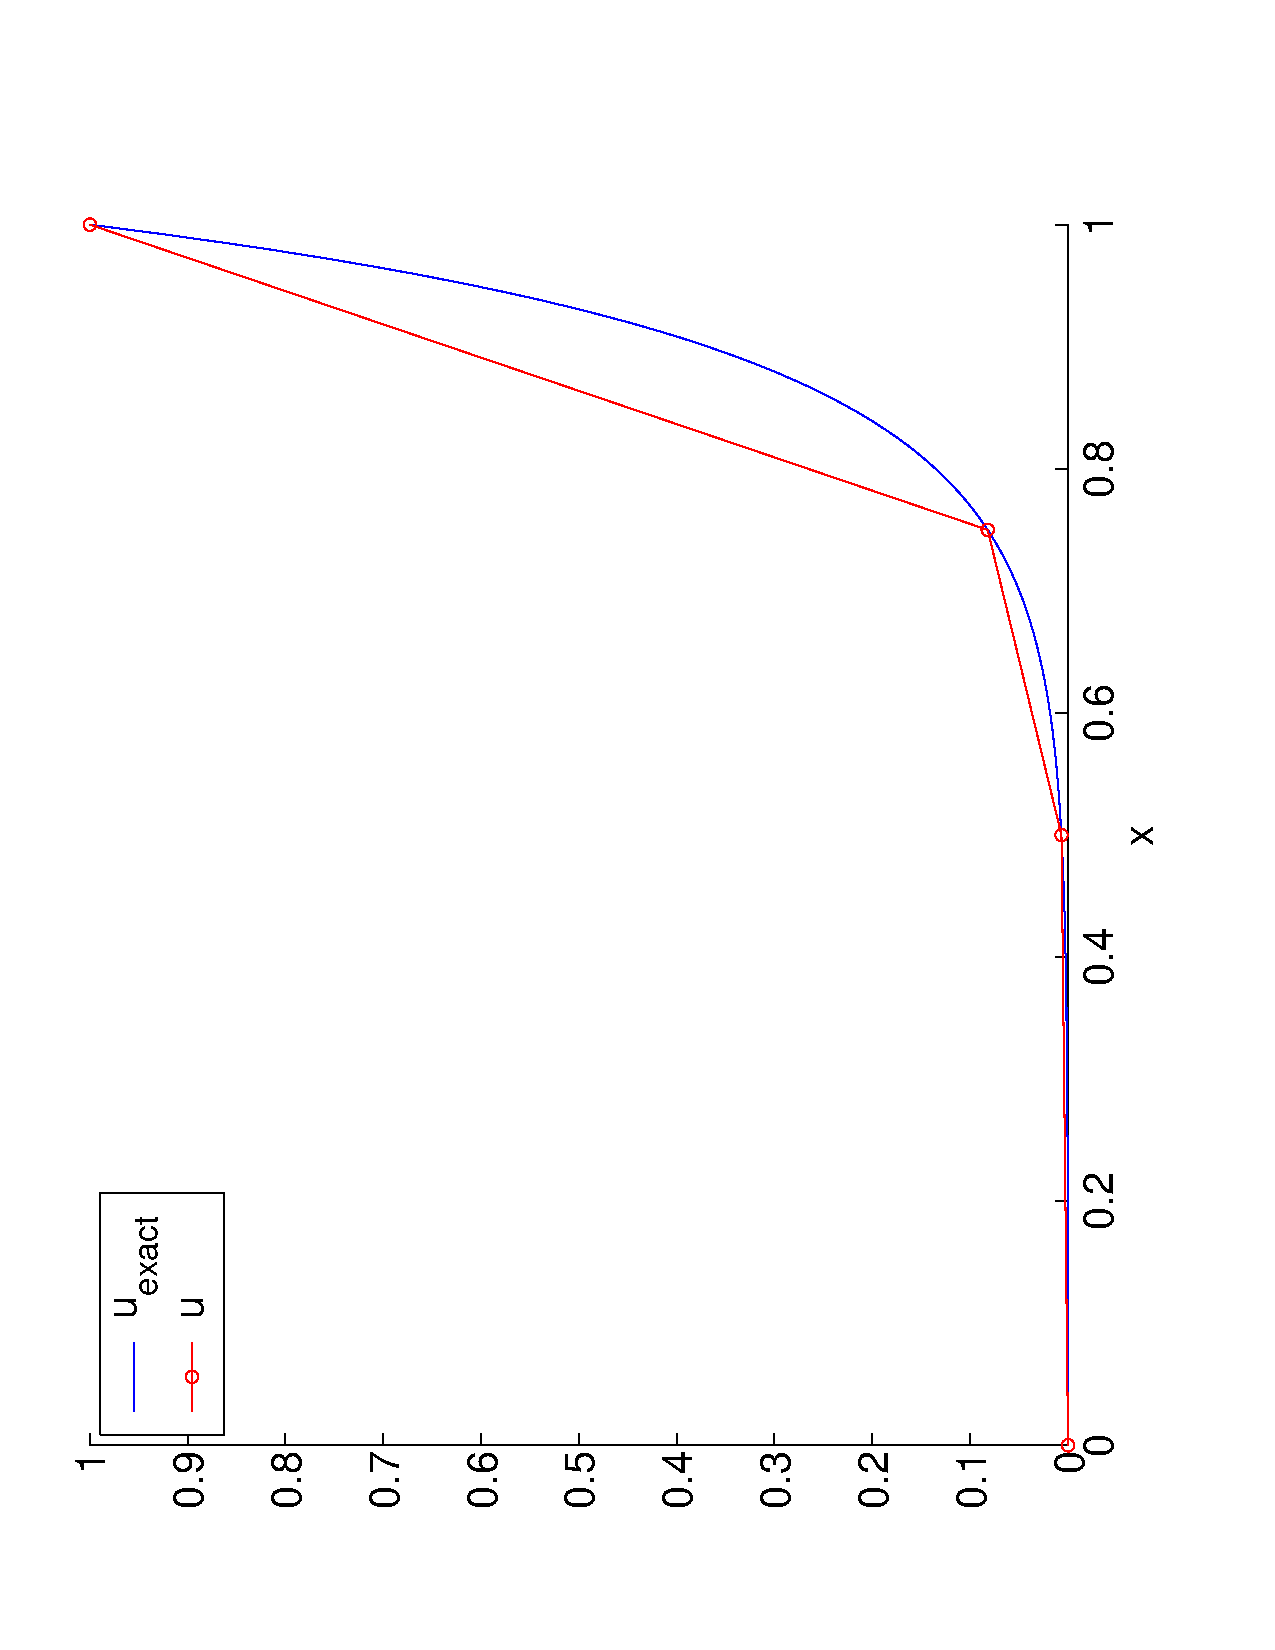
\includegraphics[width=.7\textwidth,angle=-90]{amr/adaptive_u_bl_3elems} }
  \only<3> {  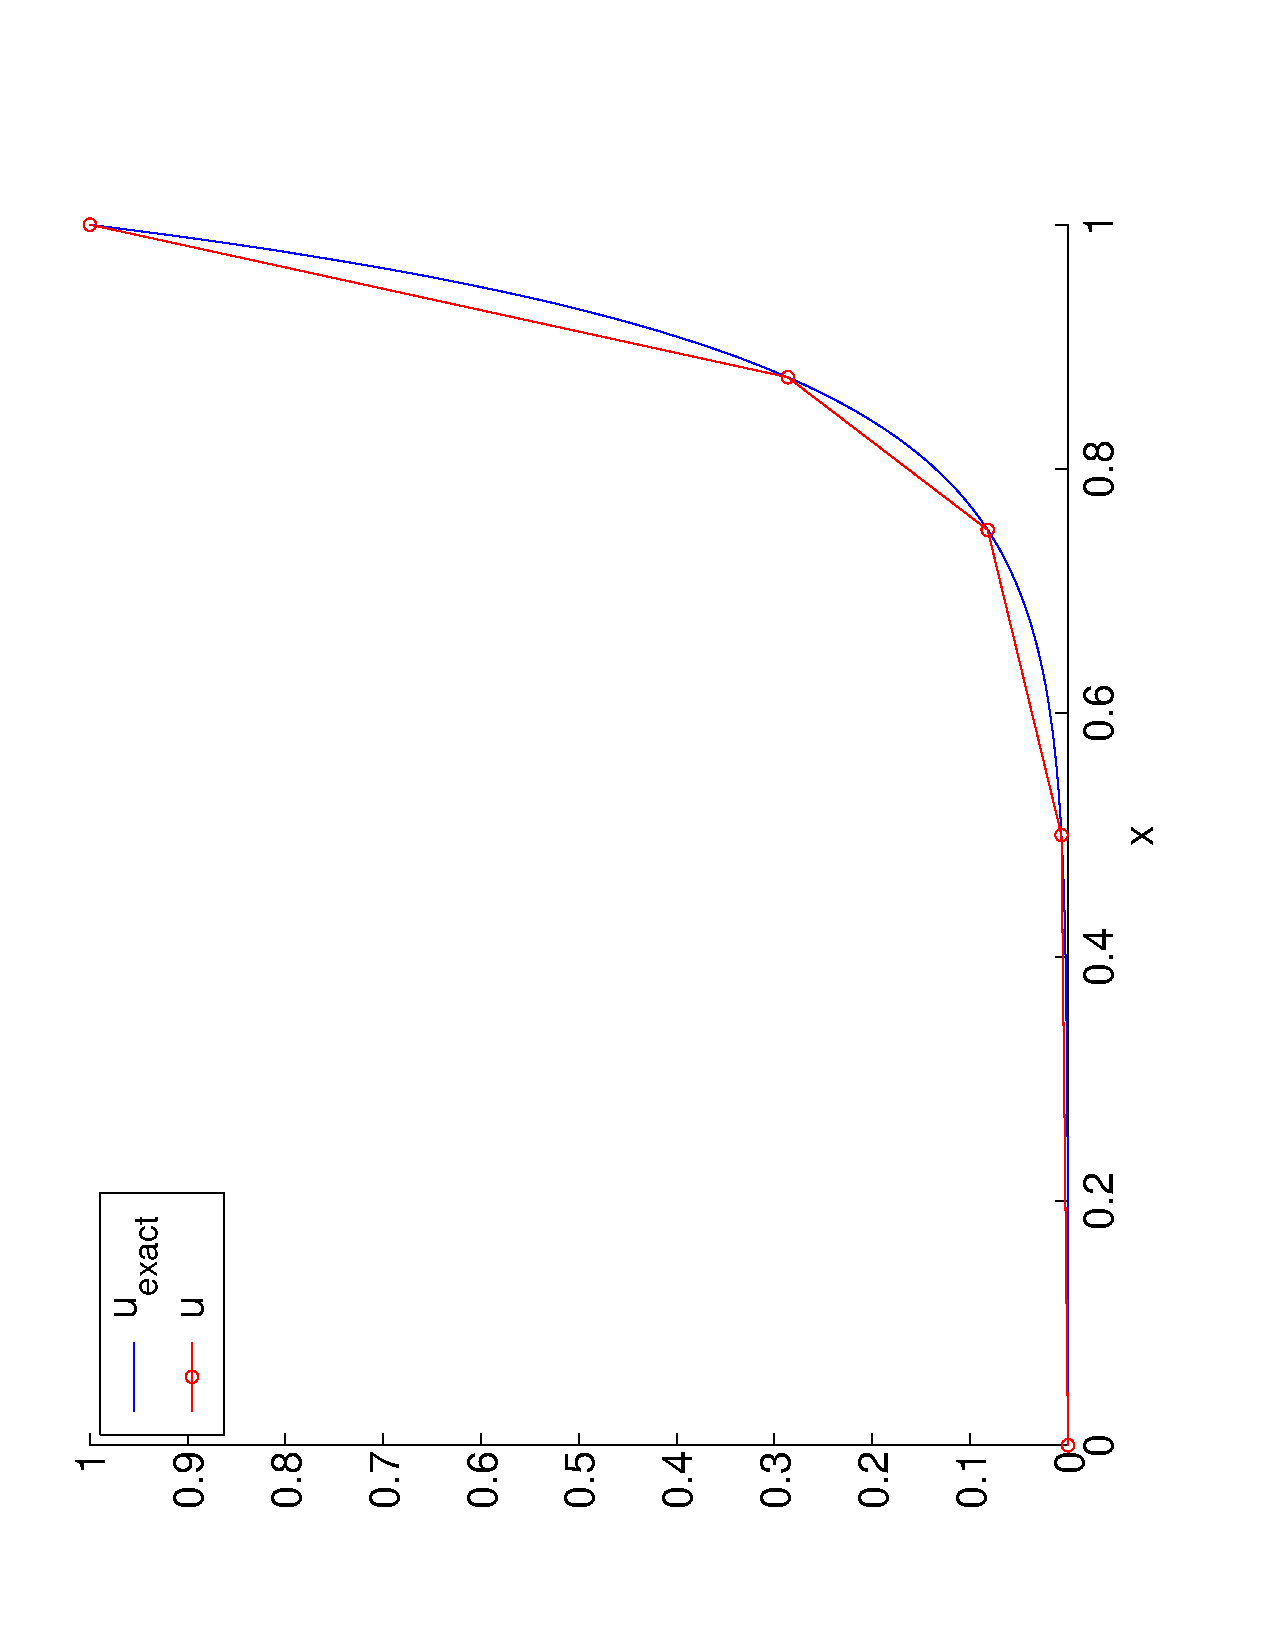
\includegraphics[width=.7\textwidth,angle=-90]{amr/adaptive_u_bl_4elems} }
  \only<4> {  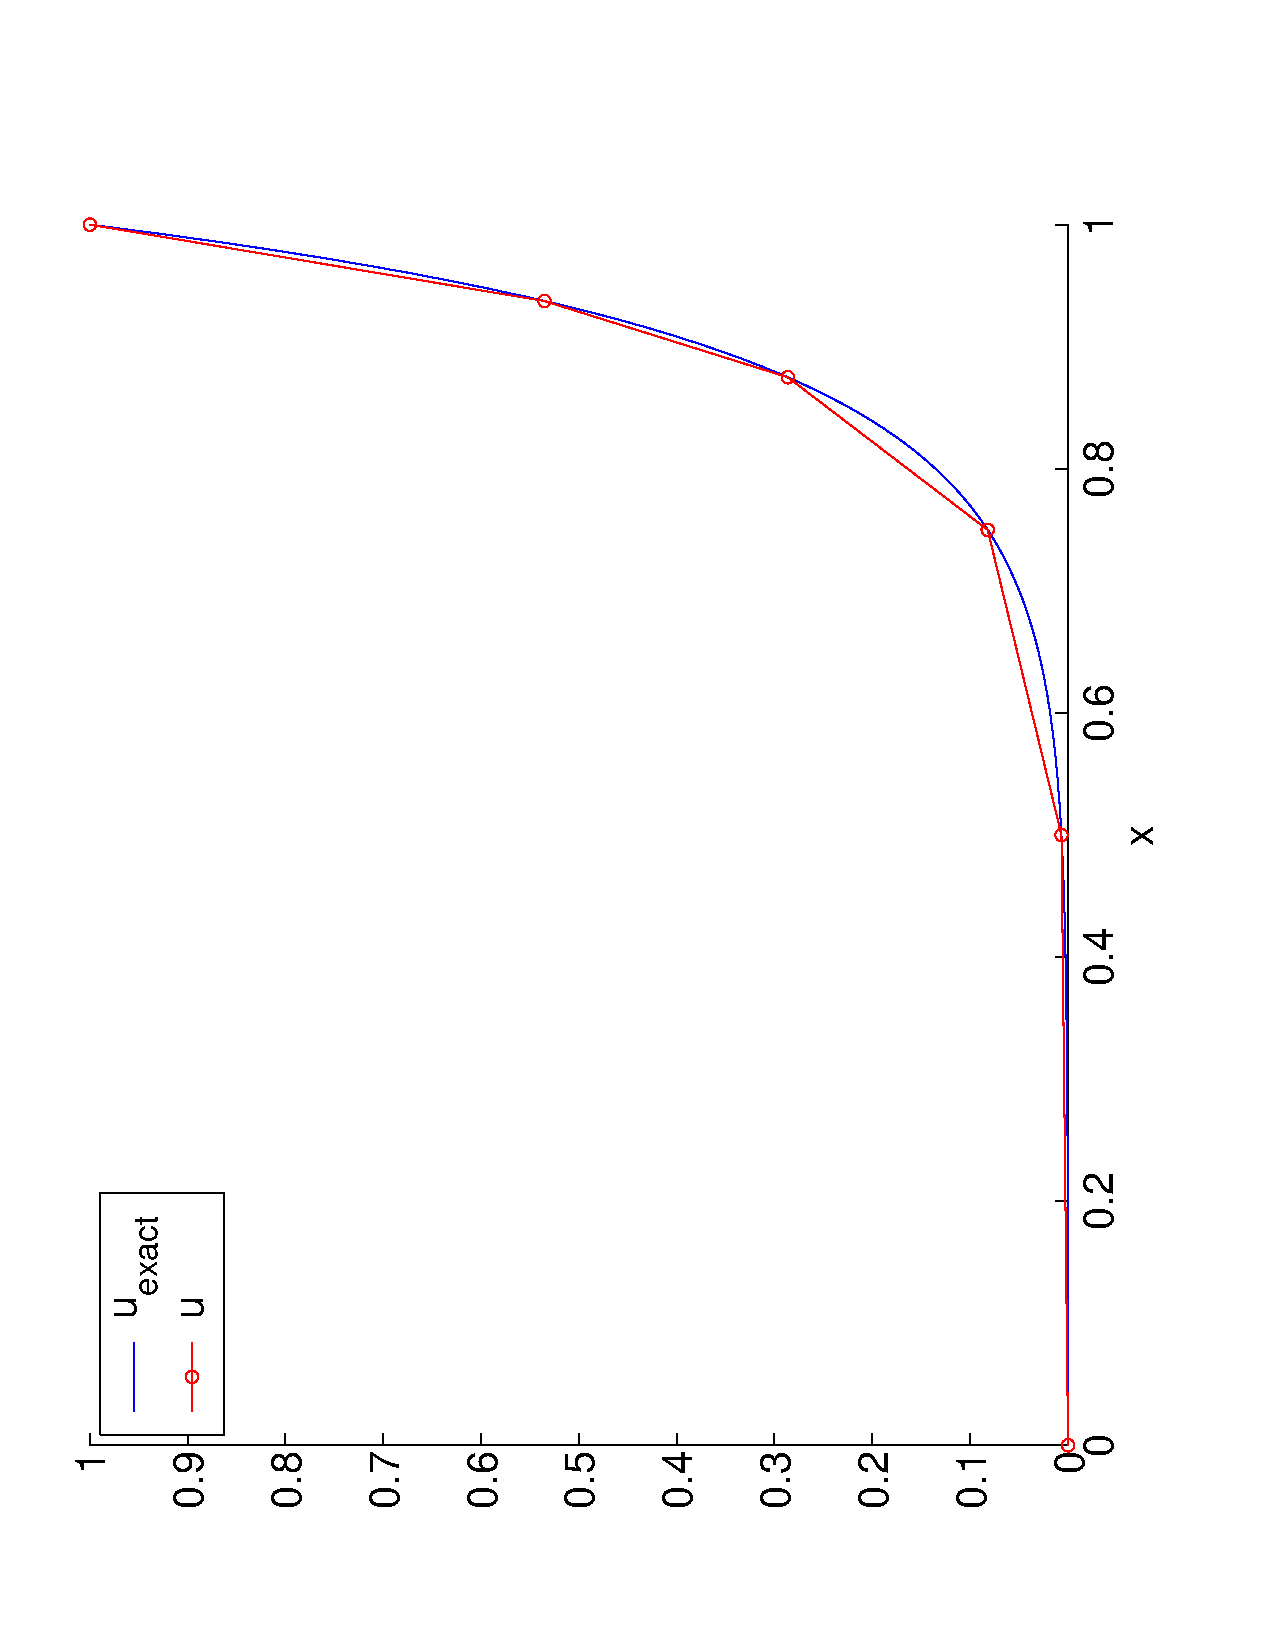
\includegraphics[width=.7\textwidth,angle=-90]{amr/adaptive_u_bl_5elems} }
  \only<5> {  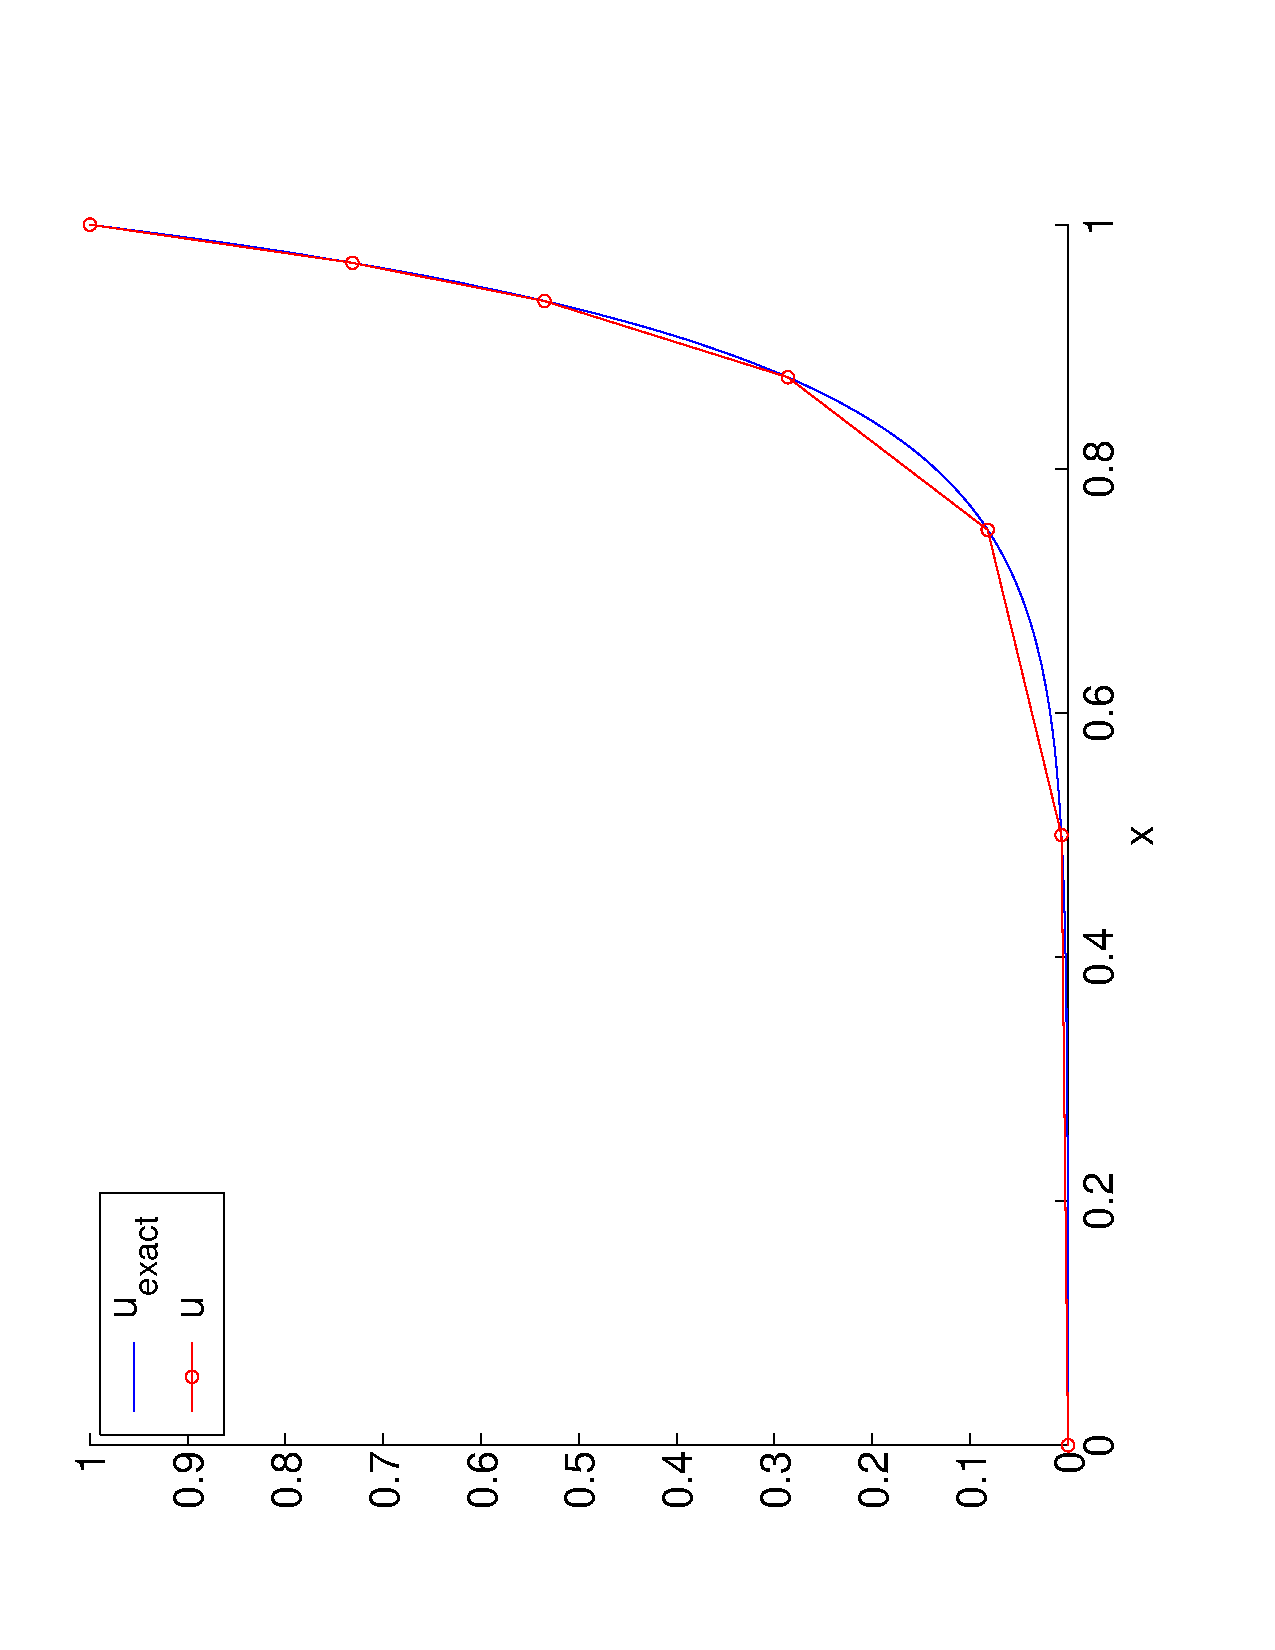
\includegraphics[width=.7\textwidth,angle=-90]{amr/adaptive_u_bl_6elems} }
  \only<6> {  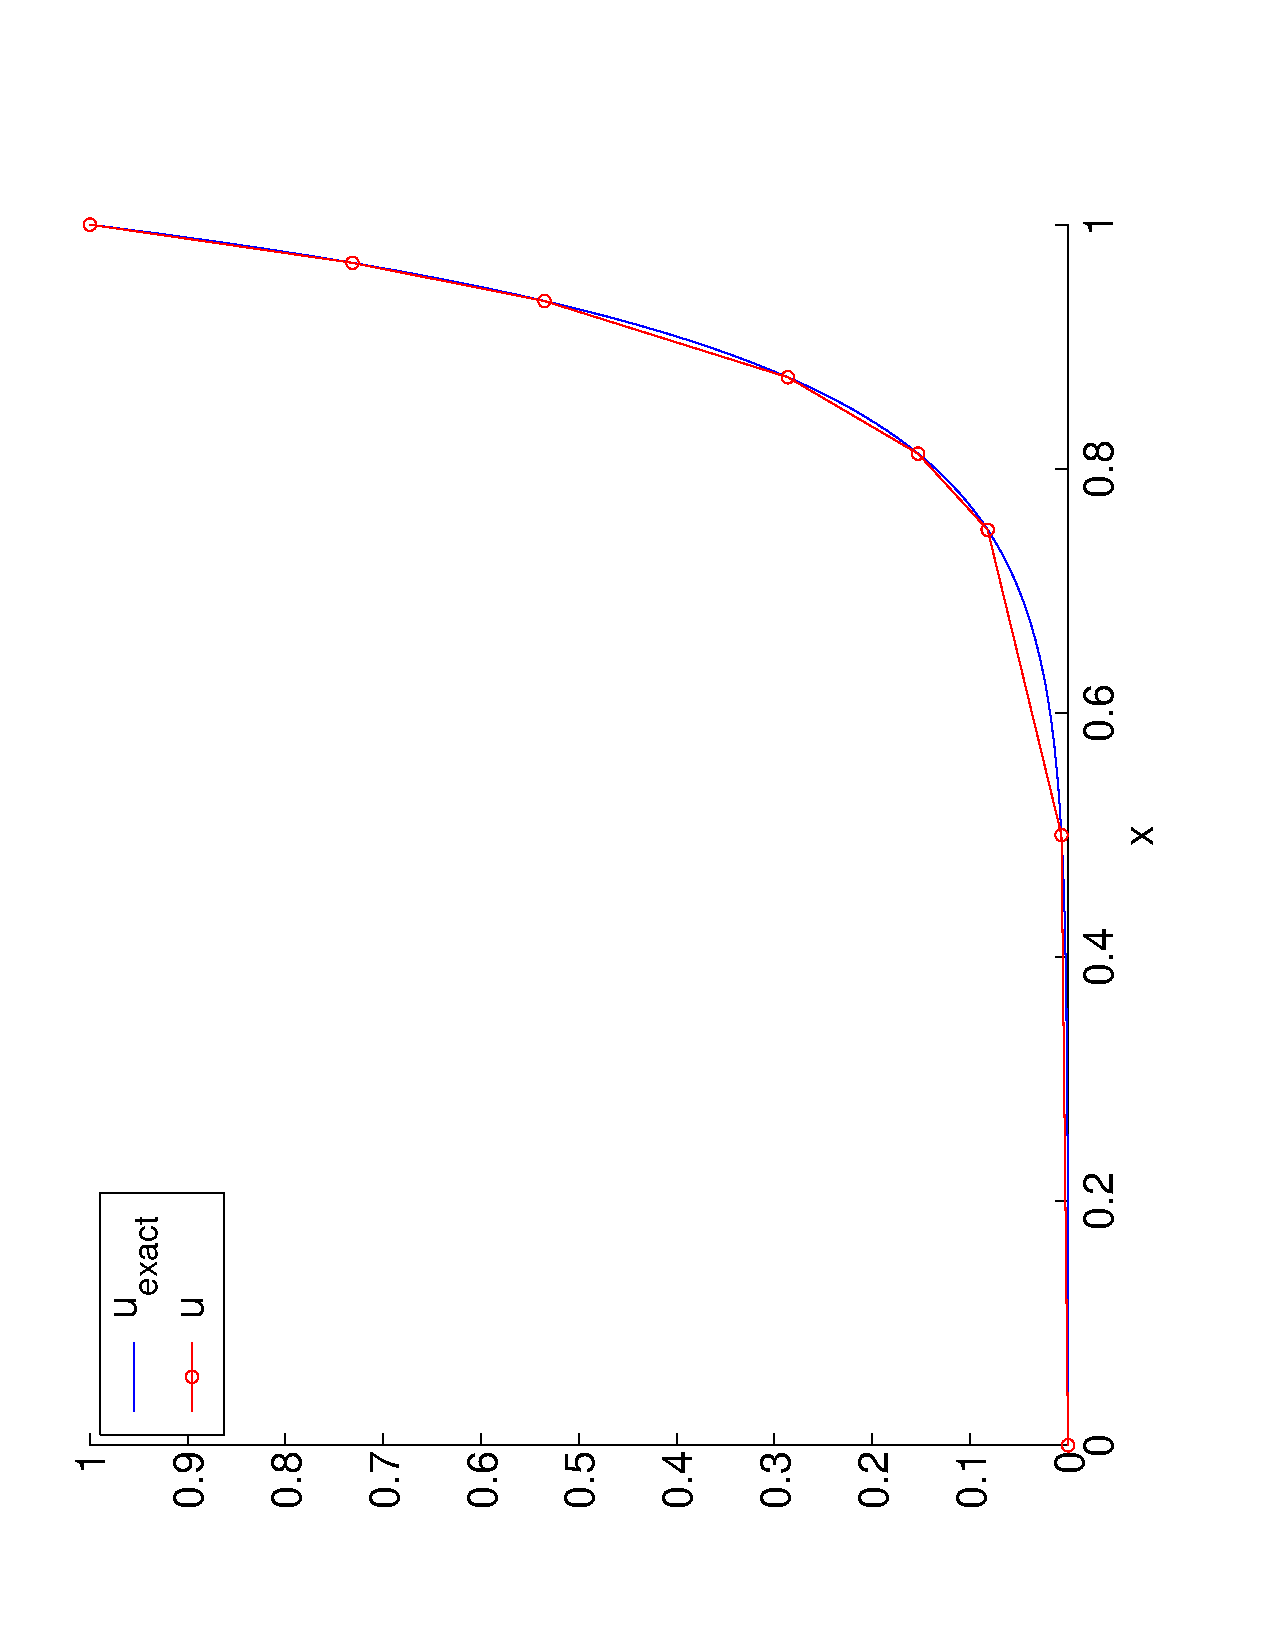
\includegraphics[width=.7\textwidth,angle=-90]{amr/adaptive_u_bl_7elems} }
  \only<7> {  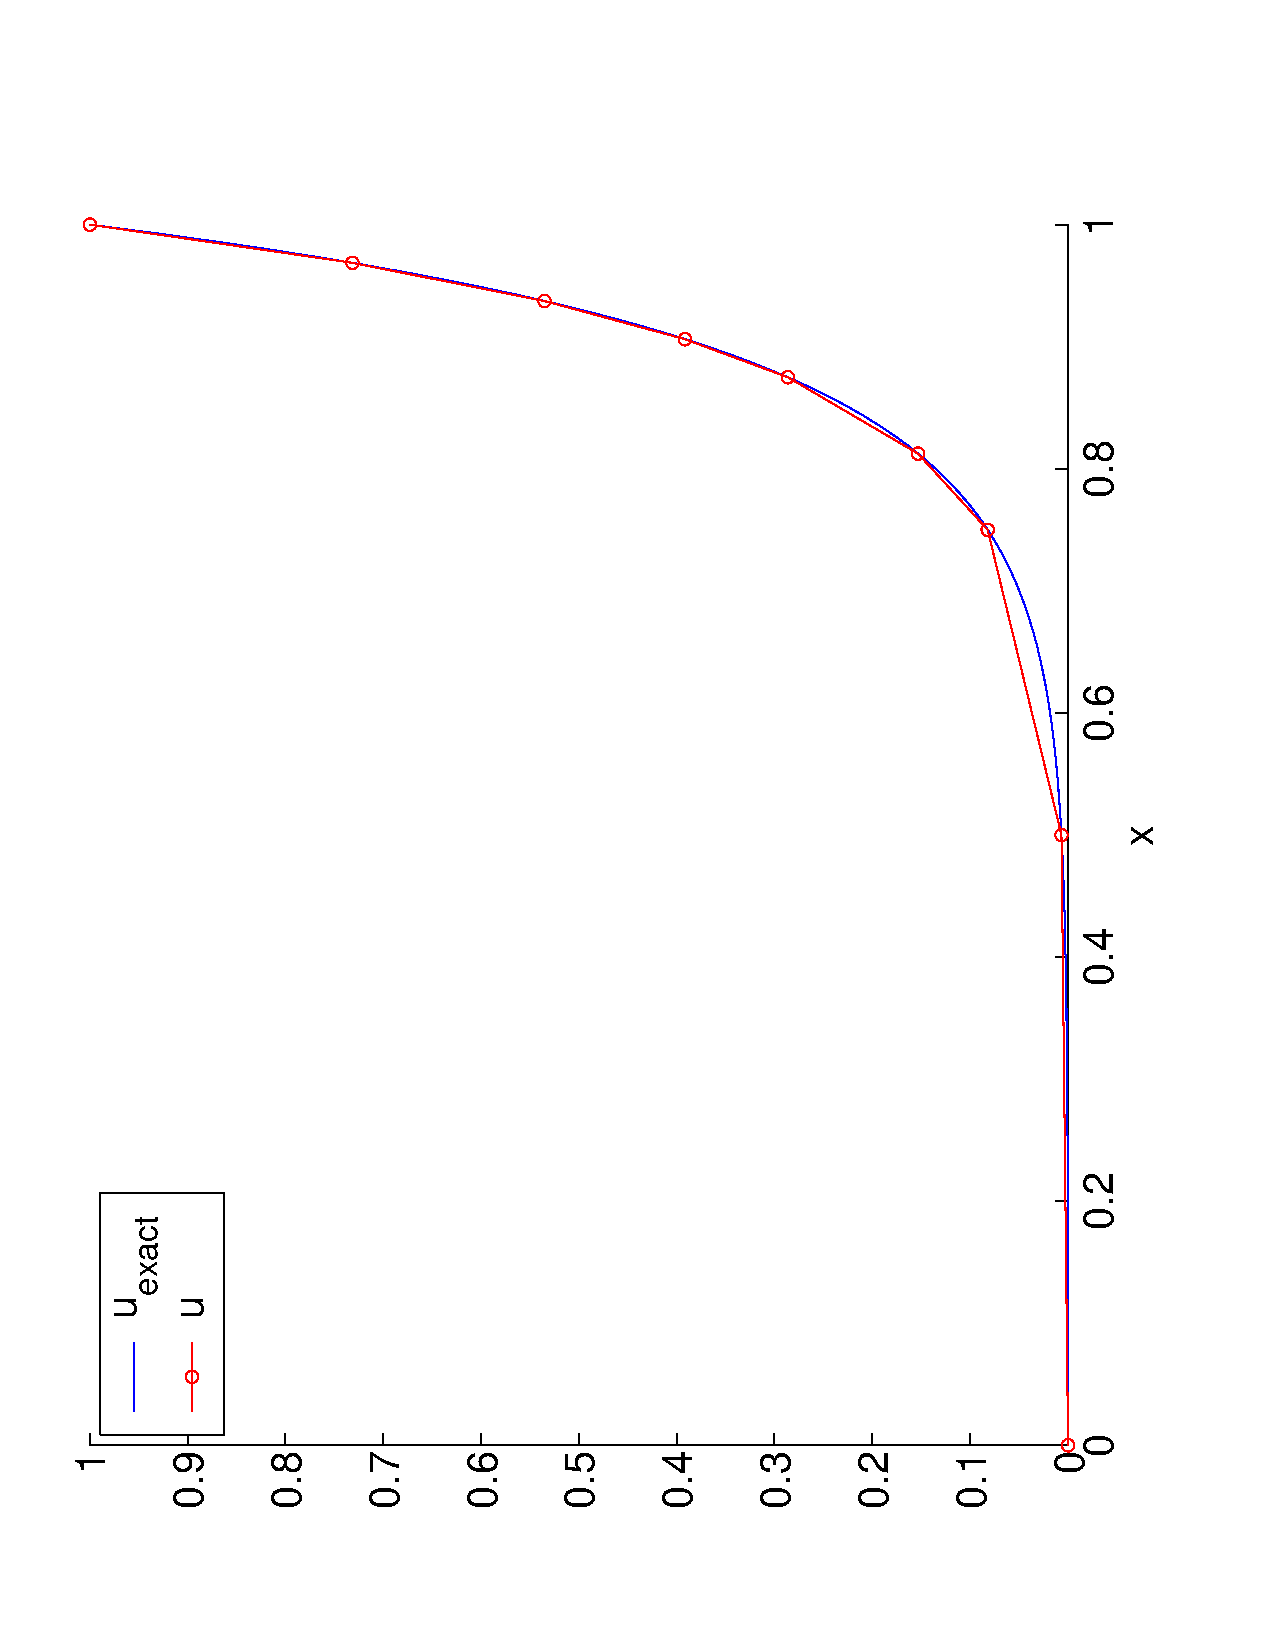
\includegraphics[width=.7\textwidth,angle=-90]{amr/adaptive_u_bl_8elems} }
  \only<8> {  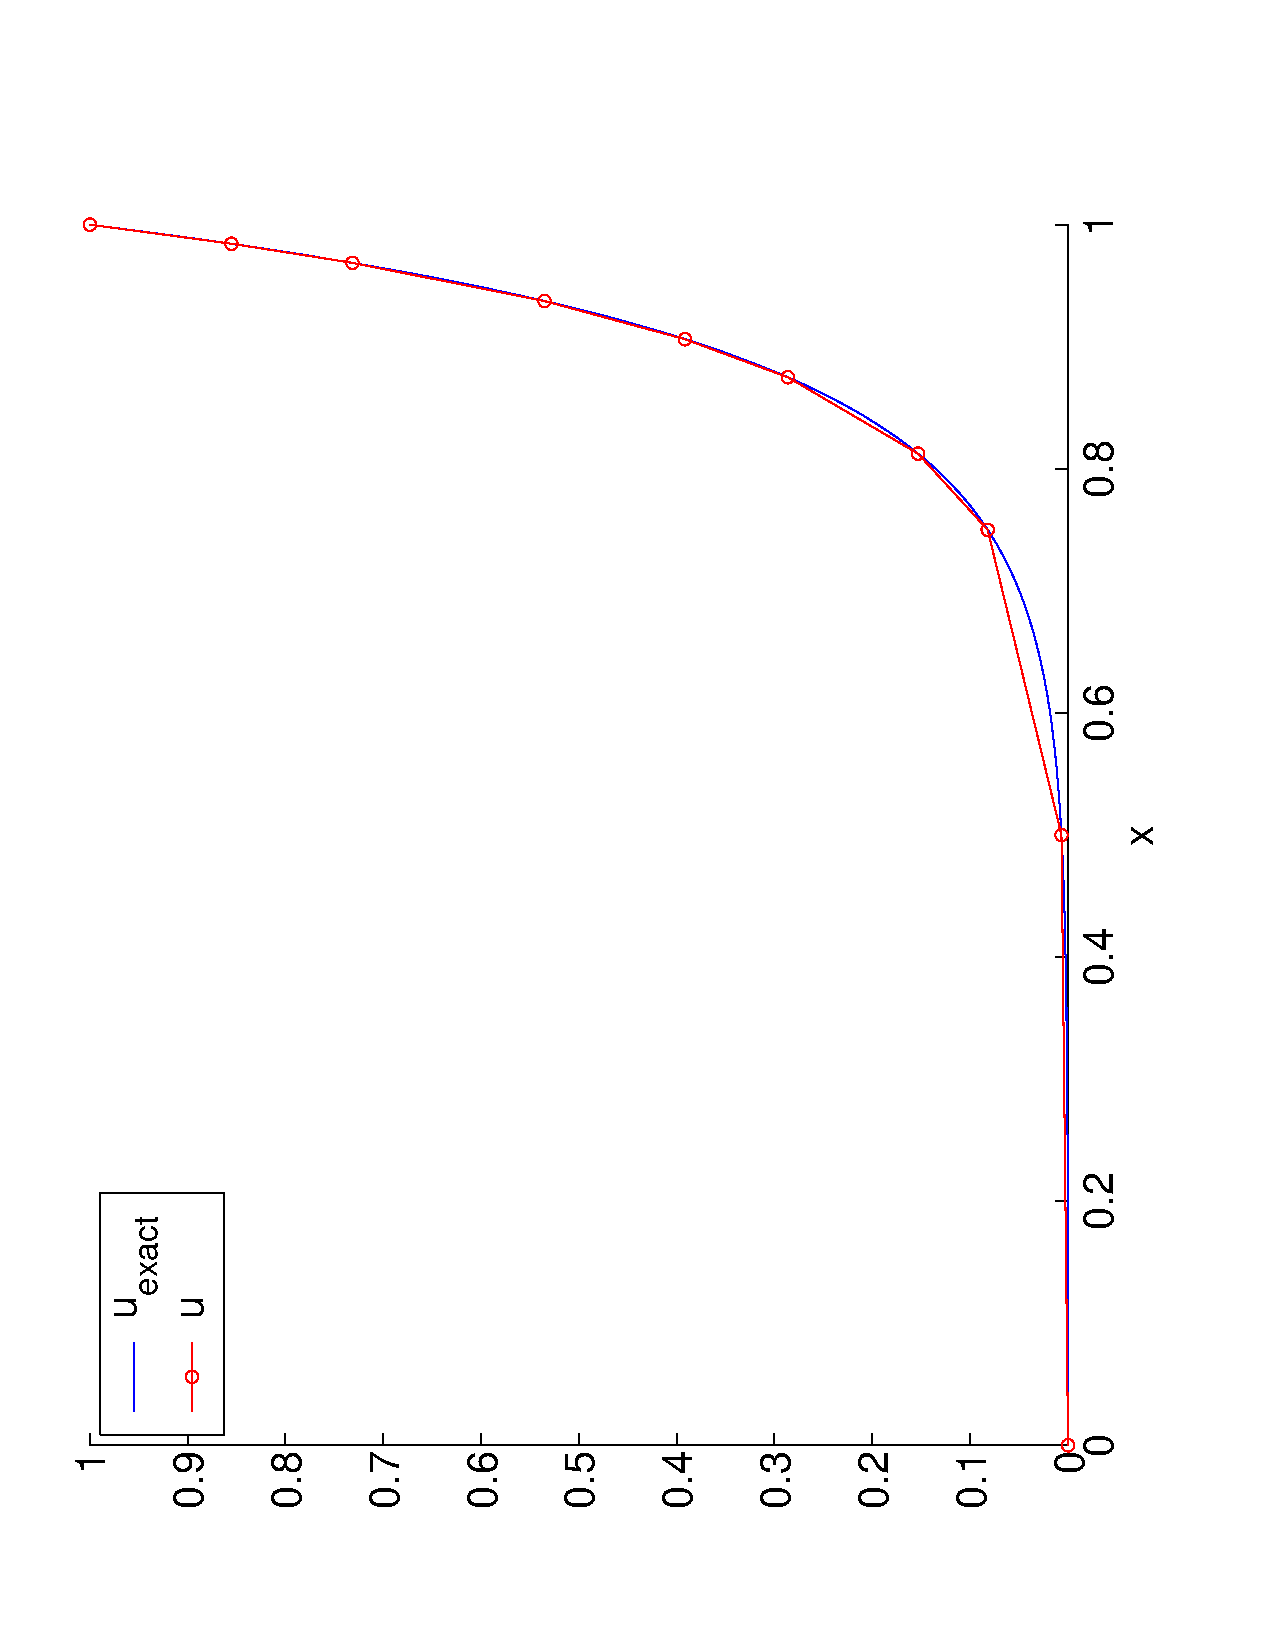
\includegraphics[width=.7\textwidth,angle=-90]{amr/adaptive_u_bl_9elems} }
  \only<9> {  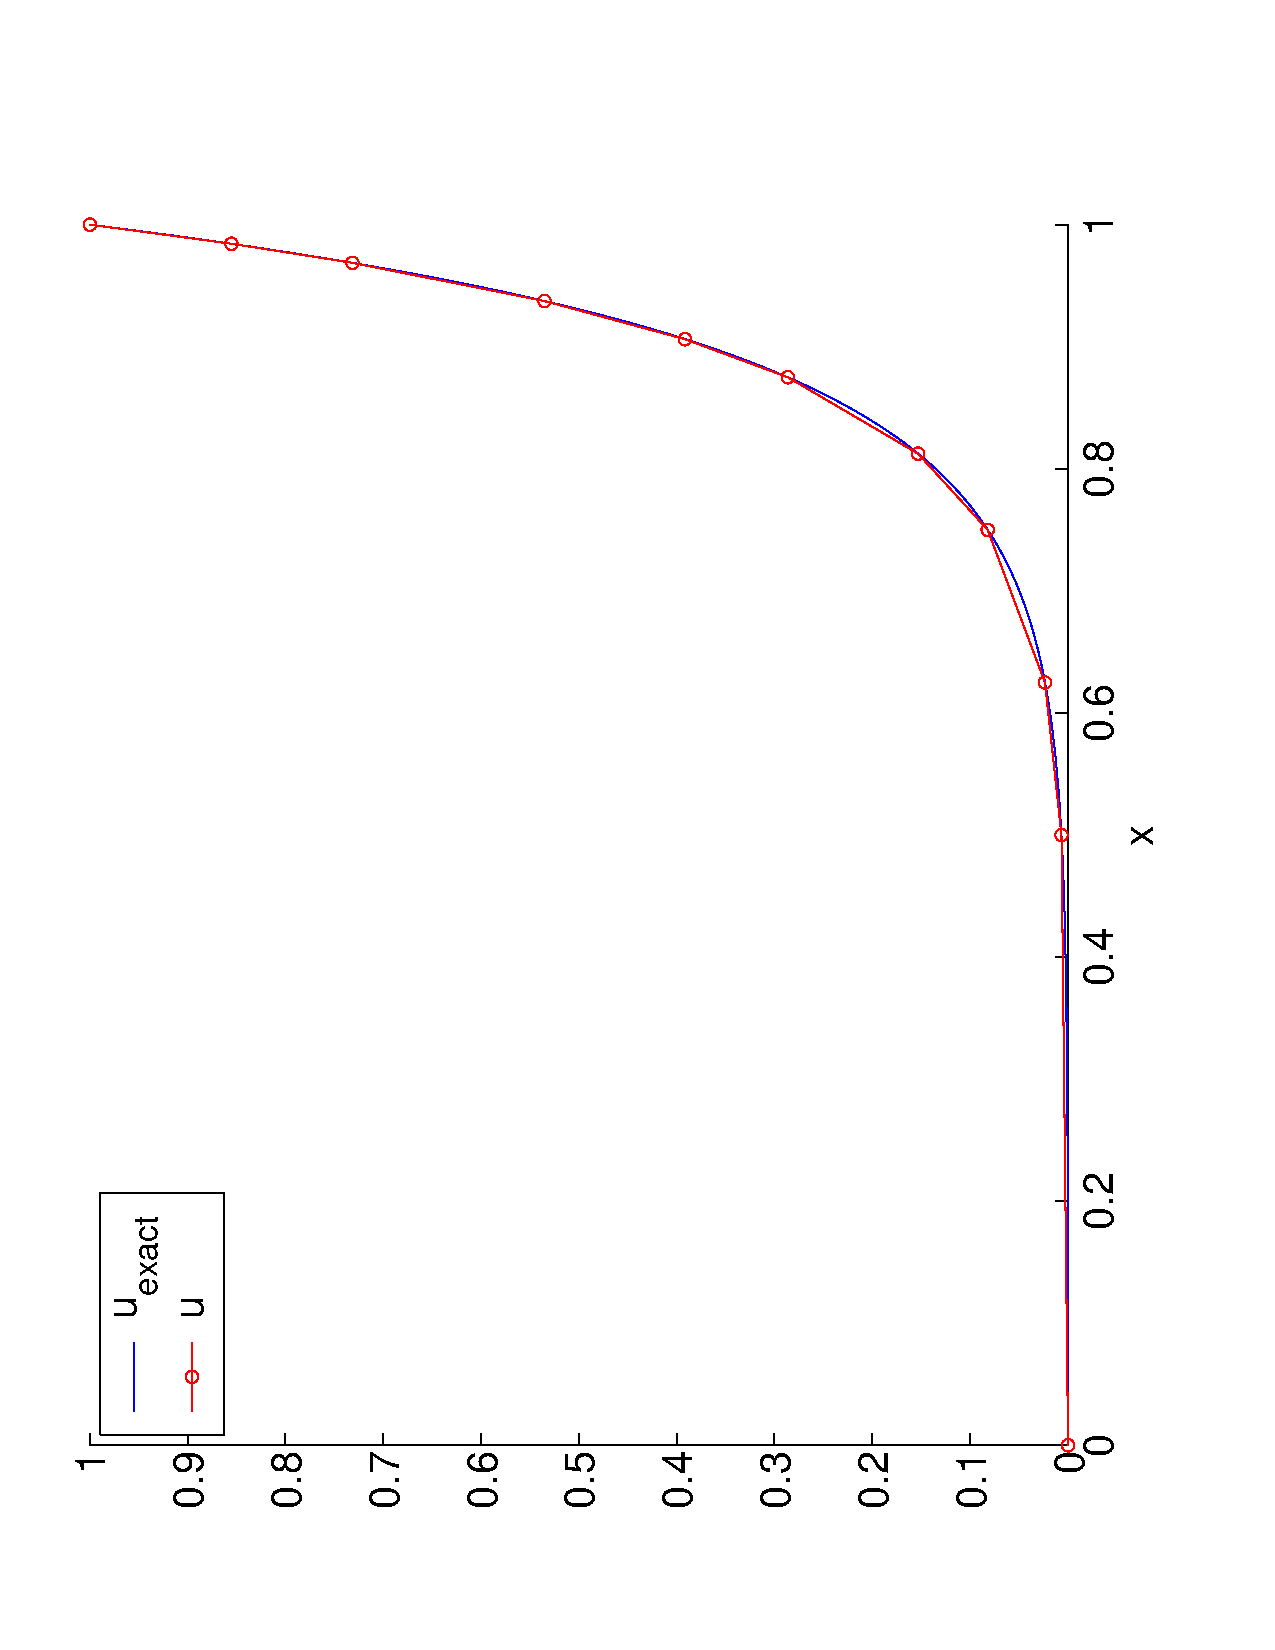
\includegraphics[width=.7\textwidth,angle=-90]{amr/adaptive_u_bl_10elems} }
  \only<10> {  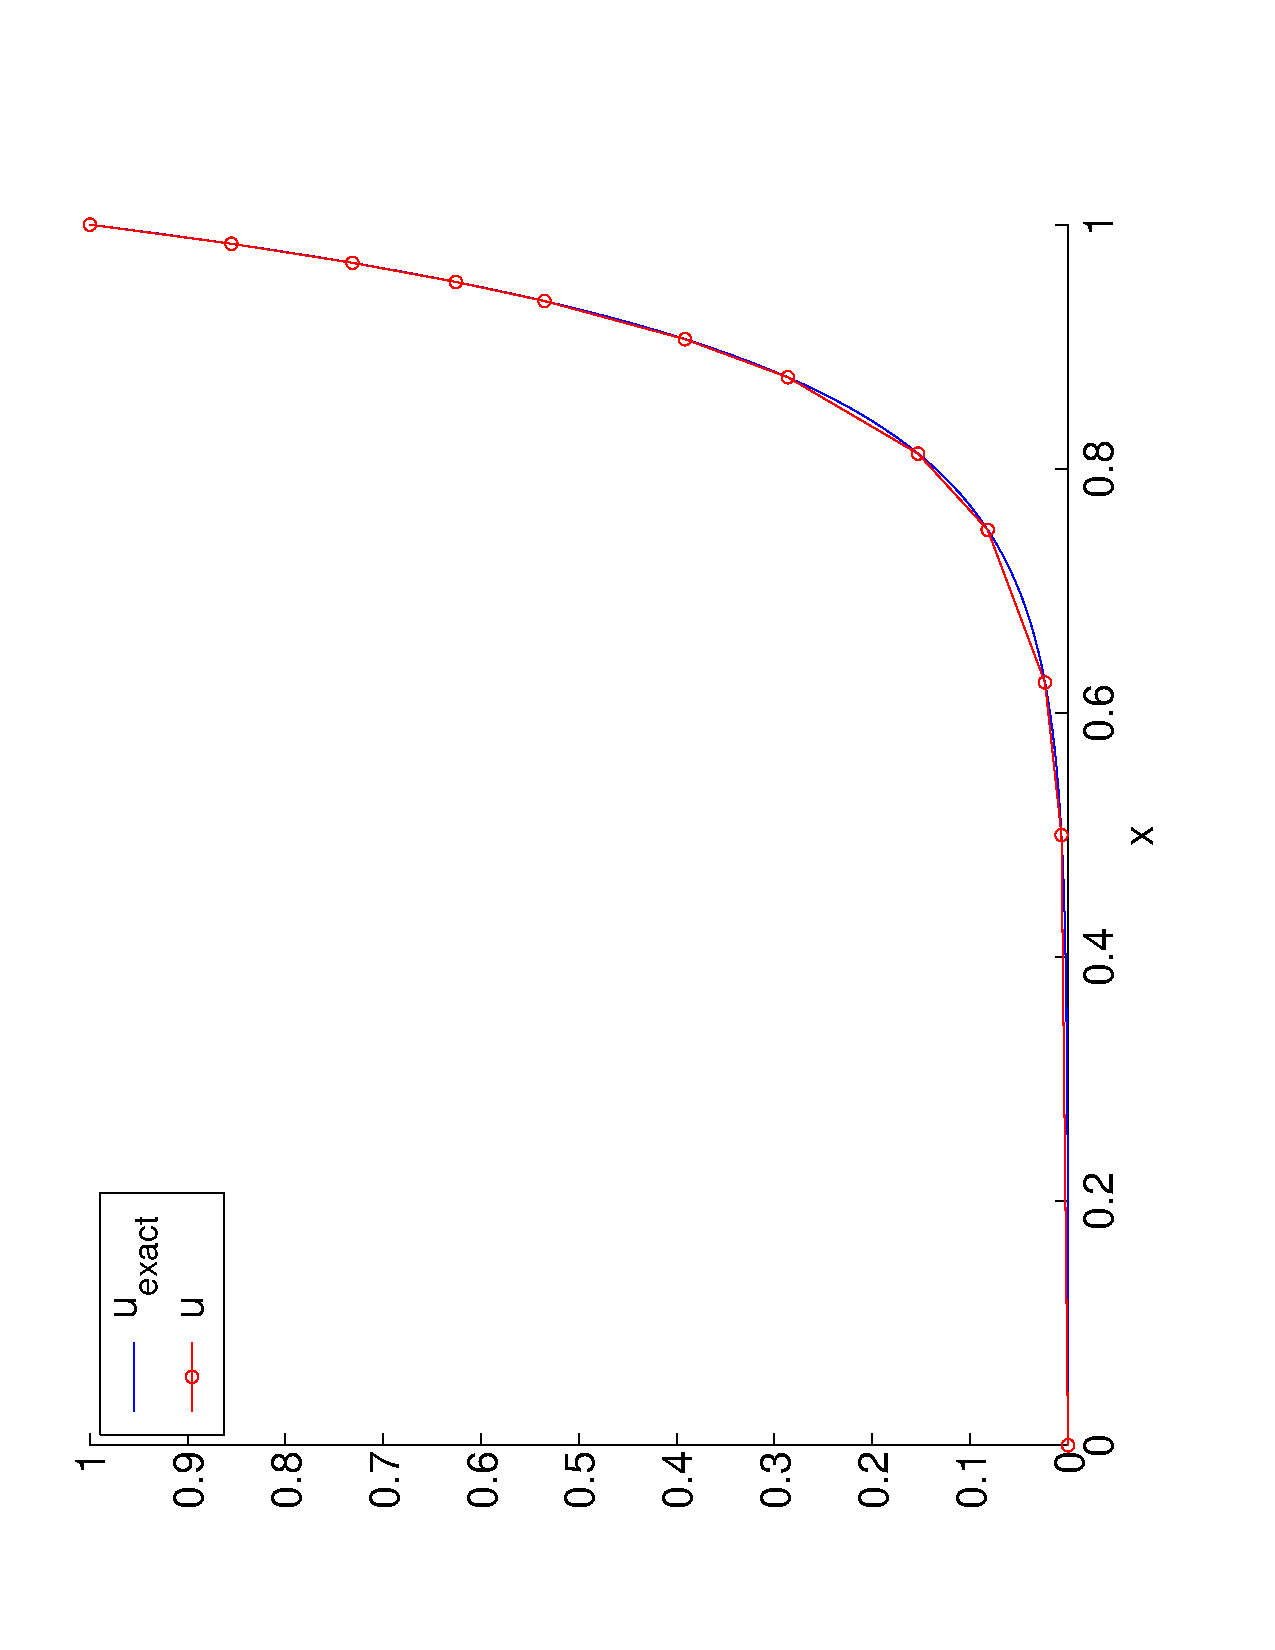
\includegraphics[width=.7\textwidth,angle=-90]{amr/adaptive_u_bl_11elems} }
  \only<11> {  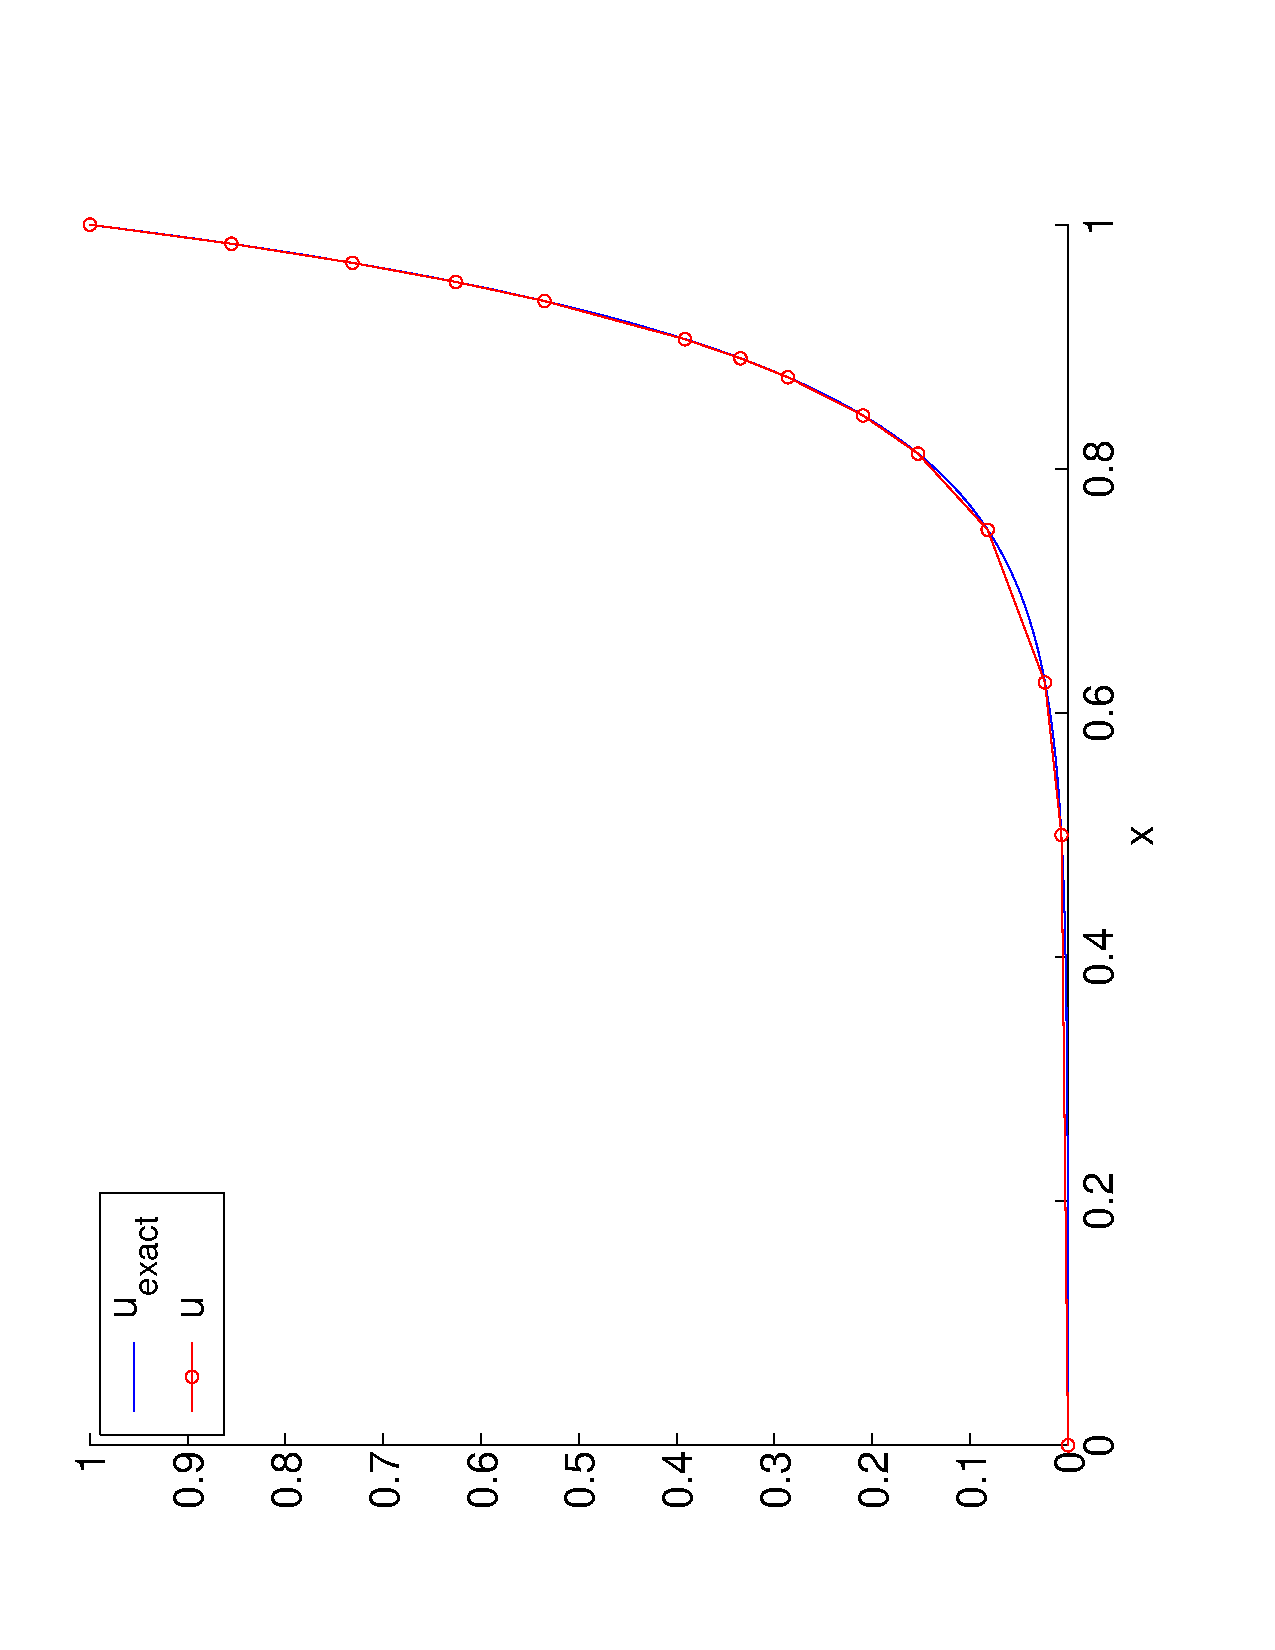
\includegraphics[width=.7\textwidth,angle=-90]{amr/adaptive_u_bl_13elems} }
\end{frame}



%%%%%%%%%%%%%%%%%%%%%%%%%%%%%%%%%%%%%%%%%%%%%%%%%%%%%%%%%%%%%%%%%%%%%%%%%%%%%%%
\begin{frame}{A Simple Refinement Strategy (cont.)}
  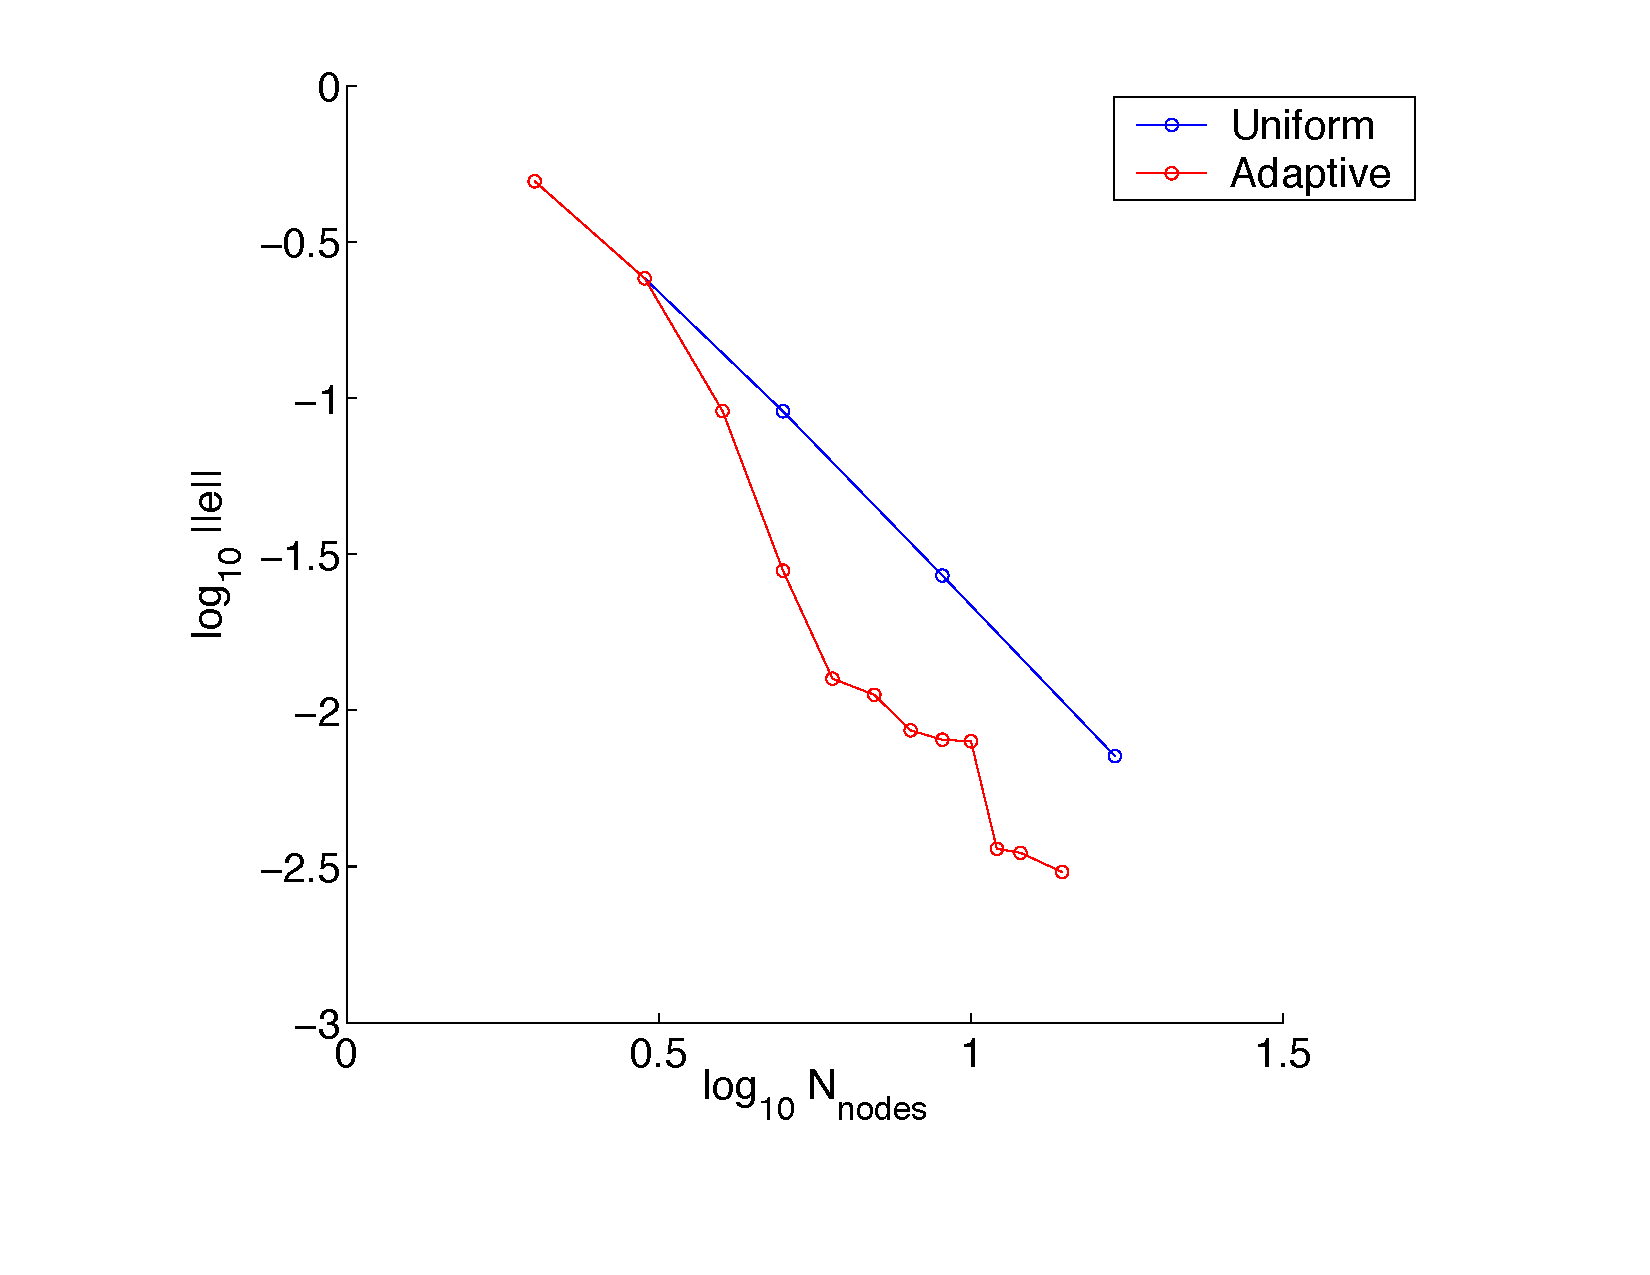
\includegraphics[height=.9\textheight]{amr/error_plot}
\end{frame}


\frame
{
  \Large
  \begin{block}{}
    \center{\bf Examples: Transient Problem with AMR}
    \center{\texttt{transient\_convection\_diffusion\_AMR}}
  \end{block}
}


\frame
{
  \frametitle{Output}
  \begin{center}
    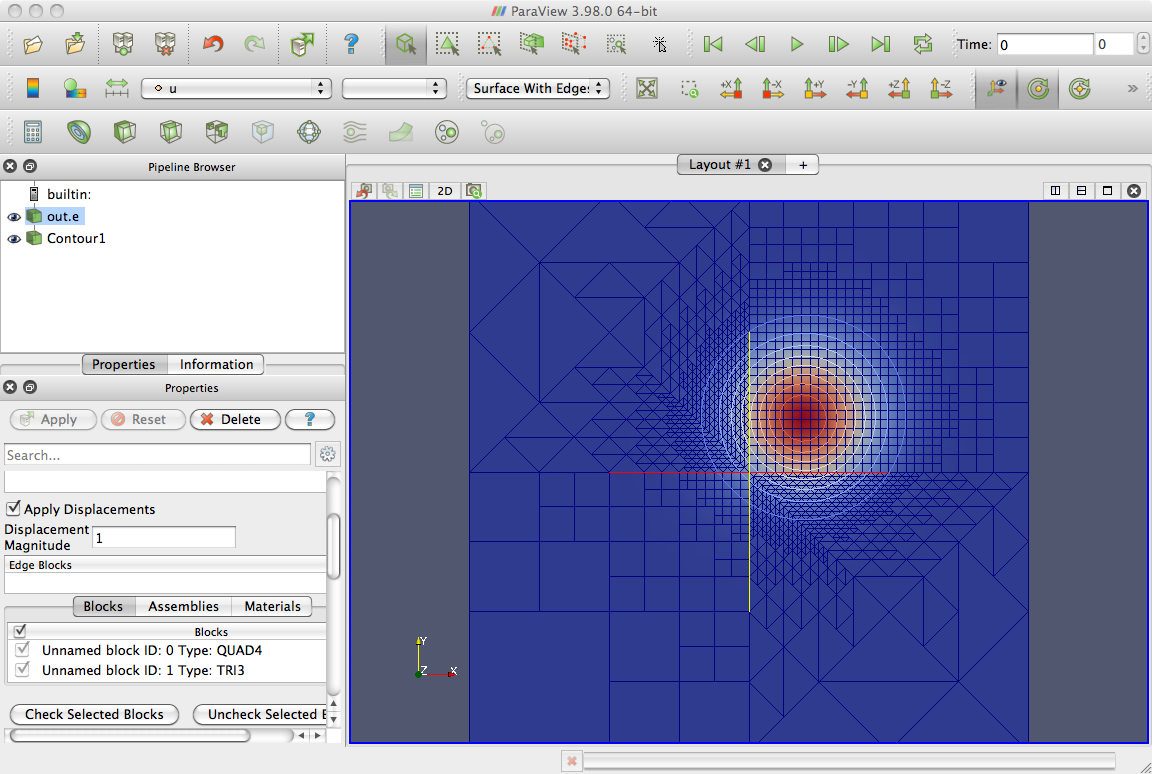
\includegraphics[height=0.8\textheight]{tutorial/transient_convection_diffusion_AMR/screen}
  \end{center}
} 

%% \end{document}

%% Local Variables:
%% mode: latex
%% End:
